\documentclass[12pt,english]{article}
\usepackage[T1]{fontenc}
\usepackage[a4paper]{geometry}
\geometry{verbose,tmargin=1.5cm,bmargin=2.5cm,lmargin=2.8cm,rmargin=2cm}
\usepackage{verbatim}
\usepackage{amsmath}
\usepackage{amssymb}
\usepackage{graphicx}
\usepackage{listingsutf8}
%\usepackage{cite}
\usepackage{array}
\usepackage{listings}
\usepackage{multirow}
\usepackage{colortbl}
\usepackage{algorithm}
\usepackage{algorithmic}
\usepackage{hyperref}
\usepackage[utf8]{inputenc}
\usepackage[T1]{fontenc}
\usepackage[main=english,greek]{babel}
\usepackage{textgreek}
\usepackage{multirow}
\usepackage{colortbl}
\usepackage{booktabs}
\usepackage{csquotes}
\usepackage{physics}
\usepackage[table,xcdraw]{xcolor}
%\usepackage{caption}

\newtheorem{definition}{Definition}[section]

\usepackage[backend=biber, style=numeric, sorting=none, compress=true]{biblatex}

\addbibresource{fsm.bib}
\lstset{basicstyle=\ttfamily}
\lstset{inputencoding=utf8/latin1}

% Adjust table row height
\renewcommand{\arraystretch}{1.5}

\begin{document}
\title{It from bit: a concrete attempt}
\author{Alexandre Furtado Neto \\ UNESP Alumnus \thanks{alexandre.com@yahoo.com, ORCID 0000-0001-9435-6566.}}
\maketitle

\begin{abstract}
This work presents a toy universe grounded in classical logic, elementary natural arithmetic, and a touch of topology. The universe’s space is modeled as a finite, closed, discrete 3-torus with an additional non-spatial dimension of a carefully selected size. Each point within this space contains a fixed-size string of two-state elements, each possessing an ontological character. A few recurring patterns are observed across these layers: one based on the Euclidean distance from a central point, the second following a sinusoidal bit mask relative to the same point, the third is a unique ray marking a privileged direction, and the fourth is a spiral path. These patterns are dynamic, relocating after interactions but keeping most data the same, displaced relative to the other layers. Time in this universe is discrete. Electric charge is represented by a single bit, weak charge by two bits, and color charge by three bits. The linear motion dynamics of the universe are dictated by a radial line of bits, while the rotational dynamics are governed by an orthogonal spiral of bits. Gravity is interpreted as an extension of the static electromagnetic force, where a certain charge combination acts as a graviton, resulting in a superdeterministic model reliant on a few input parameters. The layers, each with its hosted bubble, group as particles, either localized or similar to photons, using a fundamental collapse mechanism. Particles leave behind a trace of their momentum onto the lattice. This allows for interactions with subsequent waves, leading to patterns that resemble quantum self-interference and opening a door for falsifiability of the model. This constructive approach establishes a universal cellular automaton framework.  This work is not intended as an interpretation of Quantum Mechanics but rather an attempt to describe nature at a more fundamental level.

\medskip{}
\end{abstract}

\vfill

\begin{center}
\textbf{PACS numbers: }12.10.Kt, 03.65.Ta, 04.60.Pp, 05.45.-a
\par\end{center}

\begin{center}
\textbf{Keywords}: cellular automaton, non-locality, emerging gravity, unification
\par\end{center}

\newpage

%%%%%%%% INTRODUCTION %%%%%%%%%%

\section{Introduction}

Wheeler \cite{wheeler} coined the aphorism "it from bit." By this, he meant that anything physical—any \emph{it}—derives its existence from discrete binary choices, or \emph{bits}. This supports the notion that information has an ontological nature. The concept suggests that physics, particularly quantum physics, isn't about reality itself but is rather our best description of observed phenomena.

In this regard, cellular automata are mathematical idealizations of physical systems in which space and time, an evolution parameter, are discrete. Their attractiveness comes from the notion that simple rules can lead to really complex behavior, tending to long and interesting evolutions.

An alternative representation of the universe is developed in this work using the cellular automaton paradigm. The theme has been explored for a long time (see \cite{zuse,feynman,gardner,margolus,wolfram,fredkin,elze,Elze2019,sciarretta,thooft} for example). However, these studies generally remain in the abstract realm or present very limited models. Here, a full \textbf{3+1} core specification is posited. Although it is a qualitative analysis for the time being, the model is amenable to immediate computational investigation. We are not asserting that the universe operates strictly as a cellular automaton, but rather positing it as a convenient framework. Specifically, the representation of fundamental physical laws through the finite state machine of a cellular automaton facilitates computational inquiries. Kiefer, in \cite{kiefer2024goedel}, argues in favor of such a solution, stating that unless the spacetime structure is fundamentally discrete and the total number of degrees of freedom in the world is finite, the question of whether a given theory is the final one will remain undecidable, leaving an enduring ignorabimus.

Just classical logic and plain natural math, that is, bits manipulation, along with a hint of topology, are used in the dynamics, making up a constructive approach.

The motivation behind this initiative stems from the challenge of reconciling Quantum Mechanics and General Relativity, the two fundamental pillars of physics, into a hypothetical theory of quantum gravity (see \cite{rovelli,wald}). According to the author, this challenge arises from the presence of imaginary numbers in both Schrödinger's equation and the spacetime metric, despite their usefulness as powerful tools. Unfortunately, these very tools have created an epistemological barrier that continues to exist today.

It follows, to be clear, that, foundationally, this is not merely an interpretation of Quantum Mechanics, but rather a deeper attempt to describe nature. Notwithstanding, we recognize operator mechanics as a powerful, and perhaps unavoidable, tool for exploiting the model.

Finally, the reader will be delighted when she/he sees that purely intuitive arguments are used, leaving out obscure concepts.

The paper is organized as follows: Section \ref{sec:related-work} begins with a review of previous work in the area, followed by Section \ref{sec:space-and-time} with the foundational stage, defining the 3D space and time. Section \ref{sec:Bubbles} then introduces the bubble—the fundamental information-based element of the model. Sections \ref{sec:Particles} and \ref{initial-state} define particles, along with a description of their initial formation state. The light frame and the Finite State Machine are presented in Section \ref{sec:light-frame}. Section \ref{sec:Interactions} illustrates bubble interactions and explores the role of charge conjugation, while Section \ref{sec:Entropy-considerations} discusses the context of entropy. Section \ref{sec:Results} provides key results. Concerns about undecidability are expressed in Section \ref{sec-undecidability}, while Section \ref{sec:bridge} succinctly contemplates the bridge between the model and the QM formalism, and Section \ref{sec:Prospects-and-conjectures} outlines potential future directions. Finally, Section \ref{sec:Discussion} offers a summary and a synthetic interpretation of the model.

\section{Related work} \label{sec:related-work}

\subsection*{Stanislaw Ulam and John von Neumann}
Stanislaw Ulam, while working at Los Alamos in the 1940s, studied crystal growth using a simple lattice network, which laid some groundwork for the concept. He also suggested to John von Neumann the use of a discrete system for modeling self-replication \cite{ulam1952,vonNeumann1966}.

Inspired by Ulam's work and his own interest in self-replicating systems, von Neumann is considered the originator of cellular automata (CA) theory in the late 1940s and early 1950s. He developed a complex 29-state CA on a 2D grid to model self-replication. His work laid the foundation for much of the subsequent research.

\subsection*{Konrad Zuse}
Zuse proposed the first CA-based universe model~\cite{zuse}—the idea that the universe is a giant digital computation, laying the foundations of digital physics decades before it became a popular concept.

He suggested that space and time are discrete, and that physical processes are the result of local rule-based updates, echoing what we now call CA behavior. All of physics could emerge from information processing on a discrete grid of finite-state machines.

Zuse’s ideas inspired and legitimized later work in digital physics and CA-based universe models, influencing:

\subsection*{Edward Fredkin}
Fredkin \cite{fredkin} built upon Zuse’s vision with reversible computing. He was one of the earliest and most influential thinkers to propose that the entire universe might be a cellular automaton. His radical idea—often called digital physics or the Fredkin Finite Nature Hypothesis—suggests that reality evolves by discrete state changes, much like a cellular automaton. Space, time, and matter are all the result of information processing on a computational substrate. Everything is information.

Fredkin was a strong advocate of reversible computation, which preserves information—a key principle of both thermodynamics and quantum mechanics. He co-developed the Fredkin Gate, a reversible logic gate central to thinking about CA-based universes where no information is lost.

\textbf{Philosophical Implications:}
\begin{itemize}
  \item The universe is not just like a computer—it \emph{is} a computer.
  \item Particles are patterns of information, not physical substances.
  \item Physical laws may be \emph{emergent programs} running on a CA-like system.
\end{itemize}

Fredkin’s ideas deeply influenced Norman Margolus, Stephen Wolfram, and Konrad Zuse.

\subsection*{Martin Gardner}
M. Gardner popularized Conway’s Game of Life in \emph{Scientific American}, sparking widespread interest in CA and complex systems \cite{gardner1970}.

\subsection*{Norman Margolus}
Margolus \cite{margolus} made significant contributions to modeling the universe using CA by proposing a framework in which ``physics is modeled as a discrete, reversible, and local computation.'' He emphasized the importance of reversibility in CA to mimic physical laws. His models conserve quantities like energy and momentum, aligning with conservation laws in physics. He helped bridge computation theory and physics, influencing models of digital physics and quantum computation.

\subsection*{Gerard 't Hooft}
Gerard 't Hooft \cite{thooft}, a Nobel Prize-winning physicist, proposed a deterministic CA model as a foundation for understanding quantum mechanics. He suggested that quantum behavior may emerge from an underlying classical, deterministic system.

Quantum states are, in this view, equivalence classes of deterministic CA states that evolve in a coarse-grained manner. In his ``Cellular Automaton Interpretation of Quantum Mechanics,'' he proposes that Hilbert space formalism can be reconstructed from classical CA dynamics. Ontological states are the actual CA configurations that evolve deterministically, in contrast to quantum states, which are statistical descriptions of ensembles of ontological states.

\subsection*{Stephen Wolfram}
Stephen Wolfram proposed one of the most ambitious theories of the universe based on CA in his book \emph{A New Kind of Science}~\cite{wolfram}. His central claim is that simple rules—such as those in elementary CA—can generate complex behavior and might underlie the very fabric of the universe.

\subsubsection*{Key Contributions}
\begin{enumerate}
  \item \textbf{Simple Rules, Complex Behavior:} Even very simple CA rules (like Rule 30 or Rule 110) can produce unpredictable, complex patterns.
  \item \textbf{Rule 110 and Universality:} Wolfram proved that Rule 110 is Turing complete, suggesting that computation could be fundamental to the universe.
  \item \textbf{Computational Universe Hypothesis:} The universe evolves like a simple program, possibly a CA.
  \item \textbf{Causal Networks and Hypergraphs:} Later work, including the Wolfram Physics Project \cite{wolfram2020physics}, explores modeling space as hypergraphs, with rewrite rules updating their structure over time.
  \item \textbf{Principle of Computational Equivalence:} Most nontrivial systems are computationally equivalent—nature doesn't require special-purpose laws.
\end{enumerate}

While not a classical CA, the Wolfram Physics Project generalizes the concept: from cells in a grid to nodes in a hypergraph, and from rule tables to rewriting systems. The project remains incomplete as of 2025.

\section{Space and time \label{sec:space-and-time}}

An empirical basis for this section comes from precise measurements of the cosmic microwave background. According to the 2018 Planck results (the most recent full data release~\cite{Planck2018Parameters}), the curvature parameter $\Omega_k$ (the geometrical curvature) was measured to be:

\[
\Omega_k \approx 0.0007 \pm 0.0019.
\]
This result is consistent with a flat universe.

Let \ensuremath{L} be a huge natural odd number ($ORDER=log2(L)$ is the number of bits needed to represent this natural). Space is represented as a cluster of cells arranged in a 3-torus topology, creating a finite, closed, and discrete structure. This configuration ensures that each edge of the space seamlessly wraps around to connect with the opposite edge, maintaining continuity across the system. Additionally, an extra, non-spatial dimension forms a layered structure consisting of $W=3\cdot L^2$ layers, an odd number, with each layer containing $L^{3}$ cells. Intuitively, the value $W$ is the "cross section" of the discrete torus. \footnote{Although this spatial structure may initially resemble the classical aether—a concept once used to explain the continuity of space—it differs in that the particles, or more precisely, the fragments of particles, continuously rearrange themselves and cannot directly be characterized as a global inertial frame of reference.}

Time is treated as unidirectional and discrete, progressing in uniform steps. The extra dimension W can be visualized as extending through these layers, connecting them in a consistent, closed progression over time.

Space is endowed with memory, recording the visits of the particles, a property that will be further explored in the next section and in Section \ref{subsec:Interference}.

\subsection{The cell structure \label{subsec:The-cell-structure}}

Each cell contains the same amount of information, characterized by a bit string formatted as shown in Table \ref{tab:Cell-structure}, each possessing an ontological character. In the text, its contents will also be referred to as fragments of particles.

The input and output ports of each cell are conceptually linked through an Finite State Machine. This design choice emphasizes simplicity, as it operates using natural numbers and straightforward logical rules, steering clear of complex mathematical constructs. This finite state machine does not have the formal power of a Turing machine \cite{turing}.

\subsubsection{Physical properties}
The more intuitive variables are grouped here.
\begin{itemize}
    \item \textbf{Charge ($ch$)} \\
Defined by bit constants $q$, $w_{1}$, $w_{0}$, $c_{2}$, $c_{1}$, $c_{0}$.
Charge encompasses various discrete properties associated with the particles, derived from specific bit values that define their interactions. They are the main responsible for the emergence of forces.

\item \textbf{Route ($p$)} \\
This bit constant designates a privileged direction, serving as a foundational entity closely associated with the emergent property of momentum.

\item \textbf{Twist ($\bar{p}$)} \\
This bit constant marks the path of a spiral orthogonal to the route line. This spiral is the driver of spatial rotations and polarization.

\item \textbf{Affinity ($a$)} \\
    Groups bubbles into particles, facilitating the aggregation of smaller units into more complex entities. The affinity natural variable is essential for the formation of composite structures; without it, only a holistic universe would emerge. It is also the substrate for the emergent phenomenon of entanglement and characterizes the track left by the particles in self-interference.
\end{itemize}

\subsubsection{Wavefront shaping}
This set of variables and constants forms the mechanism for nearly perfect spherical wave propagation (with discrete constraints).
\begin{itemize}
    \item \textbf{Euclidean distance ($d$)} \\
    The Euclidean distance constant, \emph{d}, is recorded in the cell during initialization to allow precise spherical propagation.
    
    \item \textbf{Sine mask ($s$)} \\
    This bit constant represents a squared sine wave mask with a fixed period and amplitude (number of points). It serves as the basis for wave-like behavior in the system. Electromagnetic collapse only happens when this bit is true.
    
    \item \textbf{Sine timing ($\theta$)} \\
    This natural variable guides the evolution of the sine mask, functioning as an independent time variable for sine oscillations (arc).

    \item \textbf{Wavefront tick} ($t$)\\
     A clocking mechanism based on the propagation of light, governing the timing of events related to the movement of wavefronts. It is a light step counter. This long natural provides a temporal reference for activities that depend on the spread of information or interactions.
 
\end{itemize}

Variables $\theta$ and $t$ are tied as the hands of an analog clock.
 
\subsubsection{Operational variables}

This model is intrinsically nonlocal, relying on mechanisms that extend beyond conventional spatial limitations. To support this nonlocality, it employs a very rapid timing system that ensures seamless coordination across the lattice. The variables defined below are essential components of this framework, managing the dynamics of relocation, internal processes, and wavefront propagation.
\begin{itemize}
    \item \textbf{Relocation offset} ($\textbf{c}$)\\
 This natural vector determines the reissue address, guiding the position where an element is reallocated within the system. This variable controls the adjustment needed to realign or reposition bubbles in the lattice. The displacements follow the general rule
 \[
d_i = (t_i - c_i + L) \bmod L,
\]
\text{where:}
\begin{align*}
d_i & : \text{positive displacement along axis } i \, (i \in \{x, y, z\}), \\
t_i & : \text{coordinate of the target point along axis } i, \\
c_i & : \text{coordinate of the central point along axis } i, \\
L & : \text{length of the grid's side (odd)}, \\
\bmod & : \text{modulo operation}.
\end{align*}

\text{For an odd } L, \text{the coordinate of the central point is:}
\[
c_i = \frac{L - 1}{2}.
\]

    \item \textbf{Housekeeping tick} ($k$)\\
 This long natural\footnote{In this context, "long" refers to a scale on the order of $L^2$.} is an atemporal clocking mechanism, used for maintaining internal processes. It operates in coordination with the main temporal evolution, ensuring the system's consistency and directly managing important tasks.
 
    \item \textbf{Collapse flag ($col$)} \\
    A variable bit indicating the occurrence of collapse in the interaction. It is used to warn the components of a particle that a collapse occurred (see Section \ref{sec:light-frame}).

\end{itemize}

It is important to highlight the difference between $k$ and $t$. While $k$ represents the fundamental timing, being updated simultaneously in all cells at all times—each having the same value and wrapping modulo—variable $t$ is updated at each $k$ period and can take different values across layers and within different regions of a layer. Variable $t$ in fact better approaches the notion of physical time.

\begin{table}
\begin{centering}
\begin{tabular}{|l|c|l|l|}
\hline 
\textbf{\large{}Name} & \textbf{\large{}Type} & \textbf{\large{}Symbol} & \textbf{\large{}Obs.}\tabularnewline
\hline 
\hline 
\multicolumn{4}{|c|}{\textbf{Physical properties}}\tabularnewline
\hline 
charge & B6 & \emph{ch} & bits $q$, $w_{1}$, $w_{0}$, $c_{2}$, $c_{1}$, $c_{0}$\tabularnewline
\hline 
route & B & $p$ & linear motion direction bit\tabularnewline
\hline 
twist & B & $\bar{p}$ & rotation spiral bit\tabularnewline
\hline 
affinity & N & $a$ & groups bubbles into particles\tabularnewline
\hline 
position & V & $\boldsymbol{x}$ & spatial coordinates\tabularnewline
\hline 
\multicolumn{4}{|c|}{\textbf{Wavefront}}\tabularnewline
\hline 
Euclidean distance & DN & \emph{d} & for spherical constraint\tabularnewline
\hline 
sine mask & B & \emph{s} & fixed period mask bit\tabularnewline
\hline 
wavefront tick & DN & $t$ & light clocking\tabularnewline
\hline 
sine timing & DN & $\theta$ & independent time for sine (arc)\tabularnewline
\hline 
\multicolumn{4}{|c|}{\textbf{Operational variables}}\tabularnewline
\hline 
relocation offset & V & \textbf{\emph{c}} & determines reissue address\tabularnewline
\hline 
housekeeping tick & DN & $k$ & timeless clocking\tabularnewline
\hline 
collapse flag & B & $col$ & hints collapse\tabularnewline
\hline 
\end{tabular}
\par\end{centering}

\caption{Cell structure.}

{\small{}The formatted bit string is valid for all cells, where }\emph{\small{}N}{\small{}
represents a natural number, }\emph{\small{}DN}{\small{} 
a double natural number, }\emph{\small{}V}{\small{} a three-dimensional natural vector, and }\emph{\small{}B}{\small{} 
a boolean. The conventions for the values }\emph{\small{}false}{\small{} and }\emph{\small{}true}{\small{} for each 
charge bit are as follows: $q$: }\textbf{\small{}+}{\small{}, }\textbf{\small{}-}{\small{}; $w_{1}$: {[}$O${]}rbis, {[}$D${]}ark; 
$w_{0}$: {[}$R${]}ight, {[}$L${]}eft; $c_{2}$: {[}$B${]}lue, anti{[}$\bar{B}${]}lue; $c_{1}$: {[}$G${]}reen, anti{[}$\bar{G}${]}reen; 
$c_{0}$: {[}$R${]}ed, anti{[}$\bar{R}${]}ed (see Section \ref{subsec:The-cell-structure}).}\label{tab:Cell-structure}
\end{table}

\subsection{The host lattice\label{subsec:The-host-lattice}}

The space described above is occupied by three coexisting \emph{3D}-Euclidean spatial lattices made of $L^{3}$ cells each, repeated in $W$ layers (that is, $3\cdot3\cdot L^{5}$ cells total). All cells within each layer pulsate in unison, incrementing alternately the couple of evolution counters ($k$ and $t$) and exchanging information with their seven neighbors (six in dimensions $x$, $y$, and \ensuremath{z} , and one in dimension $W$, which facilitates the transfer of information between lattices and detects interactions). This exchange occurs alternately, ensuring time homogeneity is recovered every two clock ticks, grouped in four passes (see further details below), thus configuring a cellular automaton. 

The distance between cells along the three spatial axes corresponds to the fundamental quantity $X$ in the real world. The arithmetic employs $L$ as a modulus in most calculations.

The three lattices mentioned above are referred to as \textit{main}, \textit{draft}, and \textit{mirror}. The main lattice is the current lattice used in interactions; draft is the modified data; and mirror is used in comparisons of bubbles in different $W$ addresses, being modifiable too. A cell is capable of modifying its own draft and mirror cells, but not itself.

%%%%%%%% FUNDAMENTAL PATTERNS %%%%%%%%%%

\section{Fundamental patterns\label{sec:Bubbles}}

\subsection{Definition of bubble}

A \emph{bubble} is an expanding spherical wavefront of information organized across cells within a common layer. Spherical propagation is determined by comparing the Euclidean distance $d$, precomputed and stored in each cell, to the evolution parameter $t$. 

\subsection{Relocation and orphans}\label{subsec-reloaction}

Bubbles are re-emitted either immediately after an interaction or through wrapping. When the bubble is reissued, the previous wavefront continues to propagate until it fades through wrapping. In this state, the bubble is referred to as an \textit{orphan}, meaning it has affinity disabled, but is still capable of non-collapsing interactions. In this case, $a=W$ for the outer cells, set during the relocation step (see Section \ref{subsec:relocation}). The orphan does not interact with photons, because $a=W$, but interacts with gravitons (see definition in Sect. \ref{subsec:specialized-pairs}). Neutral orphan pairs do not interact electromagnetically.

A bubble can only be relocated to a point on its active surface. This guarantees that the speed of light will never be violated. Since wavefront propagation is guided by the Euclidean distance information pre-assigned to each cell, when a bubble is re-emitted due to interaction with other bubbles, all pertinent cell information must be shifted to the new position determined by the variable $\textbf{c}$. This ensures that the bubbles are relatively displaced with respect to each other. The final operation sets $t=0$ at the center cell of the relocated pattern. Relocation is the main consequence of an interaction.

\subsection{Charges and motion patterns}
Charges, or more precisely, fundamental charge fragments, are constant-valued bits that govern the interactions among bubbles. Their properties draw inspiration from the Standard Model of particle physics.

The \emph{electric} charge $q$ is associated as ever with attraction/repulsion, while the \emph{weak} charge with its two bits $w_{1}$ and $w_{0}$, or \emph{chirality}, is associated with congruence. Since the universe is closed, the addition of an extra bit guarantees this sense of congruence. The sector with $w_{1}=0$, will be called \emph{Orbis, }while the sector with $w_{1}=1$ will be called \emph{Umbra}. On the other hand, the three \emph{color} charges $c_{2}$, $c_{1}$, $c_{0}$ enforce the strong force structure. Color codes are $N:000$, $R:001$, $G:010$, $\bar{B}:011$, $B:100$, $\bar{G}:101$, $\bar{R}:110$, $\bar{N}:111$ for \emph{neutral}, \emph{red}, \emph{green}, \emph{antiblue}, \emph{blue}, \emph{antigreen}, \emph{antired} and \emph{anti-neutral}, respectively. Let signature be $sig=c_{2}+c_{1}+c_{0}$. A bubble is matter $M$ if $sig<2$, or antimatter $\overline{M}$, otherwise. Also, it is neutral $N$, if $sig=0$ or anti-neutral $\overline{N}$, if $sig=3$. The definition $color=2^{2}c_{2}+2^{1}c_{1}+2^{0}c0$ will be used in the practical implementation \cite{af_neto}.

The two path patterns formed by bits $p$ and $\bar{p}$, or \emph{route} and \emph{twist}, defined during initialization,  complement the interaction quantities. One forms a linear distribution, while the other is a spiral path.

\subsection{The sine sieve}\label{subsec:Sine}

Each layer contains an embedded squared sine amplitude, represented by a spherical mask formed by a cluster of true bits $s$  (see Section \ref{subsec:The-cell-structure}). This is a spherically uniform distribution of points modulated by the squared sine function, $sin^2(\theta)$, from $0$ to $2\pi$ radians, that is, a full period. For superimposing bubbles, the sine amplitude is independent of the primary timing variable \( t \), using $\theta$ instead, which relates to photons and other bosons whose frequencies are multiples of the fundamental cycle. The combined action of these layers forms a sieve that limits, or regulates, interactions. The density of points reflects the coupling of the electromagnetic field; that is why we used $sine^2$ instead of simply $sine$, resembling probability distributions (see Section \ref{subsec:sine-cloud}).

\subsection{Special relativity aspects} \label{subsec:special-rel}

Armed now with the concept of relocation, we can see the remarkable resemblance of the model to a Minkowski spacetime structure \cite{minkowski1909space,rindler2006relativity}.

\begin{itemize}
    \item \textbf{Light cone analogy} \\ 
    The wavefront propagation mechanism with the Euclidean distance and light step counter resembles how the light cone structure in Minkowski spacetime dictates causality and the limits of information propagation.
    The relocation mechanism updates the fragments (layers) light patterns of a particle, including the orphans.

    \item \textbf{Interval invariance} \\
    The discrete lattice preserves a form of interval invariance through its relocation rules. The displacement formula 
    \[
    d_i = (t_i - c_i + L) \mod L
    \]
    maintains a consistent relationship between coordinates, analogous to the invariance of the spacetime interval 
    \[
    ds^2 = -c^2 dt^2 + dx^2 + dy^2 + dz^2
    \]
    in Minkowski spacetime. Although the model uses natural numbers and modular arithmetic, it enforces a strict limit on wavefront propagation, echoing the preservation of causal structure. The drift of clocks is due to the presence of unequal resultants of propellers, hindering more or less the work of these devices in a fine tuning way (coincidence). Schematically we have
    \[
    \Delta \tau^2=\sqrt{(\Delta t)^2-\frac{(\Delta x)^2}{c^2}},
    \]
    where $\Delta x$ is affected by the precise amount to validate the expression.

    \item \textbf{Local interactions} \\ 
    Despite the model's non-locality at a deeper level, the reliance on local interactions within a cellular automaton framework (refer to Section \ref{subsec-reloaction}) echoes the locality of interactions in special relativity, where no superluminal communication is possible.

    \item \textbf{Symmetry considerations} \\ 
    The use of spiral for rotations bear some analogy to the rotational and Lorentz symmetries present in Minkowski spacetime, since they do not affect the metric.

\end{itemize}

%%%%%%%% PARTICLES %%%%%%%%%%

\section{Particles\label{sec:Particles}}

Bubbles form the composite structure of particles, which can be studied through experimental physics. A particle is characterized not only by the proximity of its bubbles but mainly by the fact that most of these bubbles share the same affinity value \( a \).

Two superposing bubbles can form a \emph{pair} if they share a common affinity value, $a_1 = a_2$ (see rule in Section \ref{subsec-role-of-affinity}). When two bubbles form a pair, the action of their weak or strong charges (but not the electric charge) is inhibited if they are complementary. Both bubbles are reissued in an interaction involving a pair. In general, the combinations formed correspond to boson fragments. A bubble that does not form a pair is called a \textit{singleton}.

By the simple fact that $W$ is an odd number, if we try to form pairs from different layers, an ultimate singleton will automatically remain. Let's call it the \textit{rebel}. The rebel, as we will see, will play an important role in breaking the original symmetry of this toy universe.

\subsection{Fermions}
A particle is classified as a fermion when its structure contains more than just paired kinematic components. Fermions typically exhibit a balanced average of bubbles with identical charges (the up quark is a specialized pair treated below), sustained through dynamic charge quantization (see Sect. \ref{subsec:charge-quantization}). Additionally, fermions often include pairs that act as propellers, facilitating movement. Overall, fermions form a small, undetectable volume, "punctiform" cloud of bubbles, surrounded by concentric orphans created through frequent re-emissions, thus establishing their \textit{field}.
 
Quark confinement originates from the prioritization given to color cohesion and quark-gluon interaction over other forces. In contrast, within an atom, electrons naturally distribute around the nucleus according to spherical harmonic distributions.

\subsection{Bosons}\label{bosons}
Let a \textit{blob} be a group of superposed pairs having the same affinity and the same (active) route bit.
A particle is classified as a boson if it is made of one or more blobs. Specific types of pairs that fulfill this criterion include a photon fragment and other gauge-boson fragments. Each of these roles involves a pair structure where some or all charge bits differ except for the $w_{1}$ bit; that is, they are sectorial particles. 

The defining characteristic of a photon is that all its pairs are superposed at the same point, forming a single blob. In contrast, for other bosons, such as the $W^{\pm}$ and $Z$ bosons, in which the pairs form a "punctiform" cloud of multiple blobs sharing the same affinity, somewhat similar to the behavior observed in fermions. At last, the model suggests that the Higgs boson is formed by two $Z^0$ bosons with opposite spins, with no relation whatsoever to giving mass to other particles— a rather bold claim.

\subsection{Specialized pairs} \label{subsec:specialized-pairs}

The golden rule for specialized pairs is that, unlike bosons, they do not form multi-pairs, giving them a fermionic character.

Neutrino and antineutrino pairs, $\nu$ and $\bar{\nu}$, possess color values $N, N$ and $\bar{N}, \bar{N}$, respectively. Inter-sector neutrino fragments are unique in that they do not interact via the weak force, rendering them sterile in this sense. The small mass of neutrinos is the sum of their two components and additional contributions from propellers (relativistic mass).

The up quark fragments $u$ exhibit equal, nontrivial colors and a positive charge in the case of Orbis. 

A distinct kinematic role of a pair is that of a \textit{propeller}, which continuously repositions other bubbles, forming the fundamental mechanism for inertia and motion. The propeller adds to the relativistic mass of the propelled fermion.\footnote{This reflects a Kantian view in which particles do not possess self-motion but require an external cause—here, the interaction with fragments—to change their state of motion.}

Finally, pairs that exhibit all complementary charge characteristics are termed \emph{gravitons}. These pairs can operate in both Orbis and Umbra.\footnote{Clearly, Orbis and Umbra coexist spatially.}. Each graviton pair has a fixed, absolute, oscillation frequency of 2, corresponding to their fundamental resonance in this dual framework. Gravitons contribute to the static interactions in both sectors. Without the graviton, matter from Umbra would appear entirely inert in Orbis, and gravity would not exist. The mechanism by which gravitons contribute to gravitational interactions is further elaborated in Section \ref{subsec:emergence-of-gravity}.

%%%%%%%% INITIAL STATE %%%%%%%%%%

\section{Initial state}\label{initial-state}

\subsection{Overview}
Let $S$ be the total number of states resulting from the combination of all cell values, all positions in the lattice and all bubbles. Assume there is an endless period loop $T_{P}<S$ with definite net Shannon-like entropy \cite{shannon} that corresponds to the real world. This very, very long cycle, technically a Poincaré cycle, must ideally include the initial state, ensuring no loss of information (see Sect. \ref{sec:Entropy-considerations}). Among the countless possibilities, we choose the following platonic solution for the initial state problem described below.

The initial state sets up the configuration of all cells within the lattice. At $t=0$, when all bubbles are superposed at the center ($L/2$, $L/2$, $L$/2), this state is referred to as the \textit{singularity}.

Additionally, the same initialization procedures are mirrored on the draft lattice, ensuring consistency and coherence across both structures.

Although high-level functions and real numbers are used in defining initial states, this does not violate the foundational approach of using natural numbers exclusively in the dynamic process. The real-number values and functions serve only as intermediaries for calculation, while the resulting natural number values are assumed to be imprinted directly onto the space structure by fiat. This approach preserves the integrity of a natural-number-based dynamics, grounding the system’s evolution firmly within the discrete structure of the lattice.

\subsection{Miscellaneous procedures}
First, the $\boldsymbol{x}$ vector is initialized with the appropriate Cartesian positive coordinates ($0 \dots L-1$). These values remain constant but accompany the bubble during relocation. Additionally, the time counters $t$ and $k$ are initialized to zero. The vector $\mathbf{c}$ is set to zero. 

The weak charge is defined as $w_{0}^{i} = i \,\boldsymbol{\bmod}\, 2$ and $w_{1}^{i} = (i / 2) \land 1$, while the electric charge is given by $q_{i} = w_{1}^{i} \,\boldsymbol{\oplus}\, w_{0}^{i}$. The color is determined as $color = i \,\boldsymbol{\bmod}\, 8$. Finally, all bubbles are initialized as $a_{i} = w$. These choices result in a very regular pattern of charge distribution.

This and the following pattern creation is then replicated across all layers in dimension W.

\subsection{Computing the Euclidean distance}
The Euclidean distance is a function of the spatial coordinates given by

\[
d(x,y,z)=int\left(\sqrt{\bigg(x-\frac{L}{2}\bigg)^{2}+\bigg(y-\frac{L}{2}\bigg)^{2}+\bigg(z-\frac{L}{2}\bigg)^{2}}\right).
\]
This justifies, once again, the need to adopt an odd value for $L$: a central point is necessary for this pattern to be properly defined. 

Algorithm \ref{algo:initEuclid} in Appendix \ref{sec:algorithms} shows how to apply this formula.

\subsection{Computing the sine cloud} \label{subsec:sine-cloud}
The same applies to the root sinusoidal mask, which is given by Algorithm \ref{alg:generateSpherePoints} in Appendix \ref{sec:algorithms}. In a 3-torus, the sine squared function will wrap around seamlessly in all three dimensions, ensuring that there are no discontinuities. This property allows for a continuous representation of various physical phenomena across the toroidal structure. Each dimension can be thought of as a periodic loop, where values of the sine squared function are confined within a range that recurs indefinitely. The shell of maximum amplitude must be dense (see Figure \ref{fig2}), having all its $s$ bits turned on.

The remaining subsections will compute the route and twist bits.

\begin{figure}
\centering
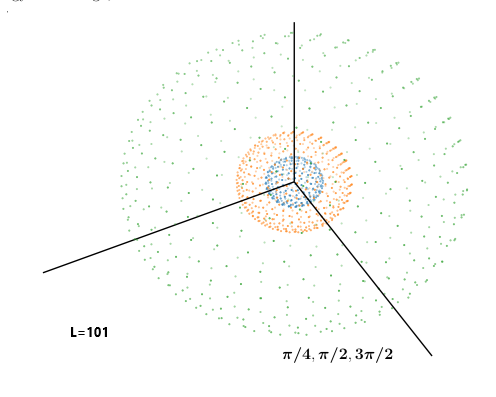
\includegraphics[width=10cm]{fig2}
\caption{The squared sine cloud.}
\footnotesize{Three shells with points distribution proportional to the squared sine are shown here.}
\label{fig2}
\end{figure}

\subsection{Computing all possible directions} \label{subsec:all-dirs}

Since the number of layers is $W$, the maximum number of possible directions is also $W = 3L^2$. On the other hand, the maximum  number of vectors is approximately $\pi L^2$. Thus, some vectors must be ignored when assigning directions to the layers. With an eye on emergent quantization, we must elect one direction as the privileged one to account for the missing directions. Let $z$ be that direction in a spherical coordinate convention. We can use a procedure based on the $sin^{2n}(\theta)$ function to constrain the vectors along $z$, where $n=1$, tentatively. Algorithm~\ref{algo:initPoleVectors} in Appendix \ref{sec:algorithms} provides this feature.

Moreover, the cases where $z > L/2$ will receive $w_1 = 0$, while the cases where $z < L/2$ will receive $w_1 = 1$, ensuring that quantization manifests itself in both \textit{Orbis} and \textit{Umbra}. Each of these vectors will be denoted as $\hat{i}'_x$ in the next subsection to construct an orthogonal basis for defining motion constraints.

\subsection{Computing the auxiliary reference bases}
The route $p$ is a constant bit used to enforce linear motion, while the twist $\bar{p}$ constant bit is used to enforce spatial rotation, as already defined. To generate the route and twist points, it is necessary to calculate an auxiliary set of three orthogonal vectors $\hat{i}'_x,\hat{i}'_y,\hat{i}'_z$, or basis. The first basis vector $\hat{i}'_x$ is tied to the route's initialization (the set $\{\hat{i}'_x\}$ was generated in the previous subsection), the second $\hat{i}'_y$ has to do with the twist, while the third $\hat{i}'_z$ will be used to define a plane to be used to build a 3D spiral that defines the twist bits themselves. Note that the bases are temporary data used to initialize the route and twist bits, which, yes, are part of the automaton. Each basis will be used to initialize one layer in the W dimension.

To ensure a consistent and uniform initialization of the route direction, each cell's route basis vector $\hat{i}'_x$ must be configured to span $4\pi$ steradians on the last shell (radius $L/2$), as stated above. On the other hand, the generation of $\hat{i}'_y$ vectors for each cell aims to ensure that they are orthogonal to the $\hat{i}'_x$ direction. This ensures that the momentum aligns with the rotational dynamics without interfering with the rotational direction defined by $\hat{i}'_x$.

If the $\hat{i}'_x$ is not aligned along a principal axis (e.g., not parallel to the $x$-axis, $y$-axis, or $z$-axis), the $\hat{i}'_x$ vector can be chosen using a simple cross product with a fixed axis to ensure orthogonality. For example, $\hat{i}'_x$ is not along the $z$-axis, set the momentum vector $\hat{i}'_y$ as: $\hat{i}'_y=\hat{i}'_x\times(0,0,1)$. If the $\hat{i}'_x$ basis vector is along the $z$-axis, the $x$-axis can be used instead to define the twist: $\hat{i}'_y$ as: $\hat{i}'_y=\hat{i}'_x\times(1,0,0)$. After computing the orthogonal $\hat{i}'_y$ vector, the two vectors are normalized and then used to calculate $\hat{i}'_z$, completing the orthogonal basis.

\subsection{Building the canonical spiral}

The canonical spiral is defined in the canonical reference frame $\hat{i}_x, \hat{i}_y, \hat{i}_z$ (the canonical route direction is the $z$ direction). It is a modified Archimedean spiral whose $z$ coordinate increases as the angle increases. The following equations are used to calculate its points:

\begin{align}
r &= \frac{L}{4\pi} \theta, \\
x &= r \cos(\theta) + \frac{L}{2}, \\
y &= r \sin(\theta) + \frac{L}{2}, \\
z &= r + \frac{L}{2}.
\end{align}

The canonical spiral (see Fig. \ref{fig3}) is then copied to each basis defined above using a rotation matrix $\mathbf{R}$, which transforms points from the canonical frame to the new reference frame. It is constructed using the rows $\hat{\mathbf{i}}'$, $\hat{\mathbf{j}}'$, and $\hat{\mathbf{k}}'$:

\[
\mathbf{R} = 
\begin{bmatrix}
    \hat{i}'_x & \hat{i}'_y & \hat{i}'_z \\
    \hat{j}'_x & \hat{j}'_y & \hat{j}'_z \\
    \hat{k}'_x & \hat{k}'_y & \hat{k}'_z
\end{bmatrix}.
\]

To rotate a point $\mathbf{p}$ in the canonical frame to the new reference frame, compute:

\[
\mathbf{p}' = \mathbf{R} \cdot \mathbf{p}, \quad
\text{where} \quad
\mathbf{p} =
\begin{bmatrix} p_x \\ p_y \\ p_z \end{bmatrix}
\quad \text{and} \quad
\mathbf{p}' =
\begin{bmatrix} p_x' \\ p_y' \\ p_z' \end{bmatrix}.
\]

\begin{figure}
\centering
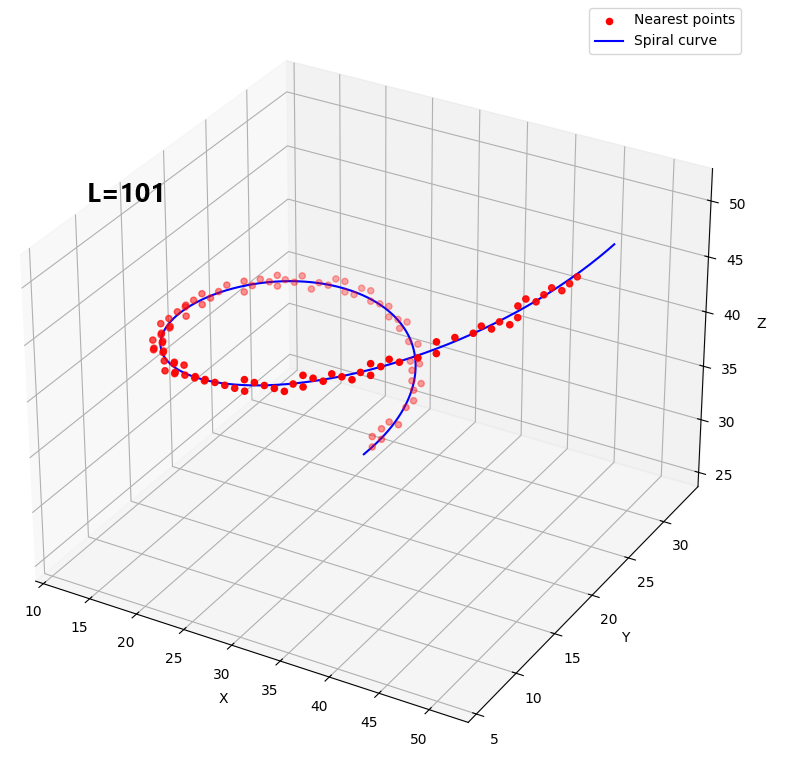
\includegraphics[width=10cm]{fig3}
\caption{The canonical spiral.}
\footnotesize{The canonical Archimedean spiral spans an angle of \(2\pi\) radians. It is replicated across each basis using a rotation matrix \( \mathbf{R} \). This path is the origin of light polarization patterns.}
\label{fig3}
\end{figure}

\subsection{Activating the route and twist bits}
Vector $\hat{i}'_x$ is then used to mark the route bits $p$ from the center to the target point, following the well-known Bresenham 3D line algorithm. 

The points forming the spiral identify the cells that must have their twist bit $\bar{p}$ activated. These spiral patterns, parametrized across all layers, induce in particular the emergence of light polarization.


%%%%%%%% THE LIGHT FRAME %%%%%%%%%%

\section{The light frame}\label{sec:light-frame}

The light frame is divided into four steps: convolution, diffusion, relocation, and transport. 

\subsection{Definitions\label{subsec:Definitions}}

To give support from now on, let us define the following natural constants related to the light frame and interactions:
\begin{itemize}
\item \textbf{DIAG}\\
Defined as $ \lfloor \sqrt{3} \cdot L \rfloor$, this constant measures the diagonal length of the 3D lattice. It is useful for determining maximum interaction distances within the lattice.

\item \textbf{RMAX}\\
Defined as $DIAG/2$, it represents half the diagonal length of the lattice, setting a maximum radius a bubble can achieve before wrapping itself.

\item \textbf{FMAX}\\
Set to $RMAX/2$, this constant represents the maximum number of superimposed bubbles that can coexist in the lattice. It ensures that the amplitude of the sine wave mask remains meaningful by limiting the interaction between overlapping bubbles. This is crucial for maintaining the integrity of the wave propagation and preventing distortions caused by excessive overlapping. It is used for consistency check only, and is supported by the Sampling Theorem \cite{Shannon1949}.

\item \textbf{CONVOLUTION}\\
Represents the convolution window, defined as $W$. This constant determines the range in which the initial convolution process is performed during the light cycle.

\item \textbf{DIFFUSION} \\
Defined as \(CONVOLUTION + W - 1\), this constant specifies the maximum diffusion range along the \(W\) dimension during a collapse event. It acts as a preparatory step for relocation if any collapse bit is true at the start, then by the end, all layers are aware of an imminent collapse.

\item \textbf{RELOCATION}\\
This constant, defined adding $(L-1)$ ticks to the diffusion step, specifies the region dedicated to bubble relocation after initial interactions and diffusion have taken place. It ensures that any necessary adjustments to the positions of particles are made.

\item \textbf{TRANSPORT} \\  
This constant, defined by adding \(3\cdot (L-1)\) ticks to the relocation step, complement the relocation process in the event of inertial transport.

\item \textbf{FRAME}\
This constant holds the same value as $TRANSPORT$, but its semantics differ. It represents the total duration of the light step, encompassing all phases: convolution, diffusion, transport, and relocation.

\end{itemize}

\subsection{Interaction principles}
Even before considering the light frame itself, let us discuss a few guiding principles adopted.

\subsubsection{Wavefronts clash}
The wavefronts of the interacting bubbles must be active. That is, the expression $d_1 = t_1 \wedge d_2 = t_2$ is true.

\subsubsection{Aggregation and dissolution}\label{subsec-role-of-affinity}

As bubbles interact, they may aggregate by sharing a common affinity, thereby forming particles. The general rule is: the smallest affinity value prevails. When particles dissolve, they assume their layer indices $a_1 = w_1, \, a_2 = w_2$. If the interaction is between a singleton and a pair, then the pair takes the affinity of the singleton $a_2=a_1$.

\subsubsection{Charge conjugation}

Charge conjugation is a principle that governs interactions between bubbles in the CA. Charges impose specific constraints on one another, ensuring that interactions occur in well-defined ways, ultimately aiming for neutrality.

Neutrality can be defined either for an isolated bubble or for a pair of bubbles. For electric charge, represented by a single bit, neutrality can only be established for a pair of bubbles with opposite charges, resulting in net neutrality. Since an isolated bubble contains only one electric bit, neutrality cannot be defined in such a case.

For weak charge, represented by two bits, neutrality arises from how the pair of weak bits combines to determine handedness in both the \textit{Orbis} and \textit{Umbra} sectors.

In the case of the strong force, which utilizes three bits, inner neutrality corresponds to the state \(000\), while inner anti-neutrality corresponds to \(111\). A pair of bubbles with complementary color bits (e.g., \(101\) and \(010\)) also exhibits net neutrality.

The general rule for interactions is then that the resulting combination of charges must achieve a neutral state.

\subsubsection{Static interactions}
The static interactions, namely the Coulomb and magnetic forces, happen through the direct alignment of a singleton, in general from an orphan wavefront, with a graviton. When the graviton interacts with the electron, it is reissued at that point. That is, the graviton is a central piece in a static interaction. Gravitons are reissued along the way of a singleton, active or orphan, increasing the probability of interacting with an electron in that region, becoming one of its propellers (see Sect. \ref{subsec:Coulomb-interaction} for more details).

It is suspected that this alignment mechanism imposes the exact filtration necessary to emulate the electromagnetic coupling constant $\alpha$, without the need to dilute the sine sieve in Section \ref{subsec:sine-cloud} by the exact ad-hoc factor
\[
\alpha\approx\frac{1}{137}.
\]

\subsubsection{Relocation options} \label{subsub:options}
When two bubbles interact, four relocation options are possible:
\begin{enumerate}
\item Both are relocated to the contact point.
    \item One is relocated to the contact point, while the other to its $p$ bit cell.
    \item One is relocated to the contact point, while the other to its $\bar{p}$ bit cell.
    \item Obeying the inertial transport rules described in Section \ref{subsec:inertial-transport}.
\end{enumerate}

\subsubsection{Pair x singleton interaction}
An interaction of the form $(p_1\wedge p_2)\vee (\bar{p_1}\wedge\bar{p_2}))\wedge s_1\wedge s_2$ provokes collapse, so $col_1=1,col_2=1$. In the other cases, the interaction is triggered by the singleton's route bit.

\subsection{Convolution} \label{subsec:convolution}
Convolution is the first step in the light frame. It contains the main interaction rules. During this phase, the mirrored image of the main lattice generated in the swapping phase (Section \ref{subsec:updating}) is used as follows. Each site is compared to its neighbor in dimension $W$, in a circular fashion. One important condition is that the cells must be active wavefront cells ($t=d$). Algorithm \ref{algo:convolution1} in Appendix \ref{sec:algorithms} shows the main logic adopted. Also during this step, as the pairs are being identified and stacked, the angle $\theta$ that selects the squared sine point density is incremented accordingly. This angle reflects indirectly the notion of frequency.

In the convolution step, the formation (or reformation) of particles occurs.

The comparisons are divided into two main groups: the bubbles are superimposing, or the bubbles have distinct origins.

\subsubsection{Superposing bubbles}
Two overlapping bubbles can form a pair if they satisfy the following conditions:
\begin{itemize}
    \item They both have frequency equal to one, $\theta=t$.
    \item Their combination is not forbidden by these rules:
    
\begin{align}
    &\left( c0_a \wedge c1_a \wedge c2_a \wedge c0_b \wedge c1_b \wedge c2_b \wedge q_a = q_b \right) \notag \\
    &\vee \left( \neg c0_a \wedge \neg c1_a \wedge \neg c2_a \wedge \neg c0_b \wedge \neg c1_b \wedge \neg c2_b \wedge q_a = q_b \right)
\end{align}

\end{itemize}

The formation of multi-pairs is made during this step too. Pairs are allowed to superpose if they satisfy these rules:

\begin{align}
    &\overline{q}_a = \overline{q}_b \wedge \overline{w1}_a = \overline{w1}_b \wedge \overline{w0}_a = \overline{w0}_b \wedge 
    \overline{c2}_a = \overline{c2}_b \wedge \overline{c1}_a = \overline{c1}_b \wedge \overline{c0}_a = \overline{c0}_b \notag \\
    &\Rightarrow (\text{Orbis} \vee \text{Umbra})
\end{align}

\begin{align}
    \text{Orbis} \quad &\equiv \quad (\overline{c2}_a > 0 \wedge \overline{c1}_a > 0 \wedge \overline{c0}_a > 0) \wedge \notag \\
    &\quad \big( (\overline{q}_a = 0 \wedge \overline{w1}_a > 0 \wedge \overline{w0}_a = 0) \vee \notag \\
    &\quad\quad (\overline{q}_a = 0 \wedge \overline{w1}_a > 0 \wedge \overline{w0}_a < 0) \vee \notag \\
    &\quad\quad (\overline{q}_a \neq 0 \wedge \overline{w1}_a > 0 \wedge \overline{w0}_a < 0) \big)
\end{align}

\begin{align}
    \text{Umbra} \quad &\equiv \quad (\overline{c2}_a < 0 \wedge \overline{c1}_a < 0 \wedge \overline{c0}_a < 0) \wedge \notag \\
    &\quad \big( (\overline{q}_a = 0 \wedge \overline{w1}_a < 0 \wedge \overline{w0}_a = 0) \vee \notag \\
    &\quad\quad (\overline{q}_a = 0 \wedge \overline{w1}_a < 0 \wedge \overline{w0}_a > 0) \vee \notag \\
    &\quad\quad (\overline{q}_a \neq 0 \wedge \overline{w1}_a < 0 \wedge \overline{w0}_a > 0) \big)
\end{align}

Net charge calculation and affinity fusion, implicit in the formulas, are done as necessary, seamlessly.

\subsubsection{Distinct bubbles} \label{subsec:distinct}
A number of potential interactions may occur when the bubbles are distinct. The algorithm referred to above shows schematically how it happens for most cases.

If two singletons have opposite charges, we have annihilation, with both bubbles being re-emitted from the contact point and their affinity receiving their default values. Both $col$ bits turn true.

If the two singletons share the same affinity, but have different charges, then the singleton whose route is the contact point is reissued from the contact point. The other bubble is reissued from the inertial-transported route.

If the charges of two singletons are equal and the route of the first bubble hits any point of the active surface of the second bubble, then we have fermionic cohesion. The bubbles receive the same affinity; the first bubble is re-emitted from the contact point, while the second from its active twist cell.

\subsubsection{Higher frequencies}
As stated earlier, variable $\theta$ dictates the behavior of photons and other bosons, whose frequencies are multiples of the fundamental cycle. This accelerated time is used to find a suitable point in the sine sieve to allow interaction, defining a concentric bubble. The point found in the sieve must then propagate to the cells in the Euclidean bubble, where $t=d$, during the Diffusion phase, because only there it can be used as a sieve.

\subsection{Diffusion}  
This phase propagates states across the \(W\) dimension if necessary. A non-trivial relocation offset \(\boldsymbol{c}\) is used to reposition the bubble in the 3D space, and the \(col\) bit is utilized during the traversal of all layers in the \(W\) dimension. If any \(col\) bit is true at the start, then by the end, all collapse bits will be true for all bubbles sharing a common affinity. The spread of the collapse bit in the \(W\) dimension is necessary for identifying all fragments that compose a collapsing particle. The sine sieve bit found in the previous section is also propagated in this phase.

\subsection{Relocation} \label{subsec:relocation}
The final part of the light step addresses bubble relocation itself. Bubbles shift in specific directions (north, west, down) until they have completed their relocation process, including the inertial transport mechanism (See Section \ref{subsub:options}).

To complete, the diffusion of the time variable $t$ occurs here at the last tick: When a cell has a neighboring cell with a lower $t$ value, it updates its own $t$ variable to match the lower value. With this rule, the relocated bubble is capable of expanding again. This timing is crucial to avoid the 'clean cube' with the new value overrunning the orphaned data.

When the relocation is complete, bubble variables are prepared for the next cycle. If the time frame completes, the $k$ counter resets to zero, preparing the system for the next iteration.  At the conclusion of the process, all $\boldsymbol{c}$ vectors will have a null value.

\subsection{Main lattice updating} \label{subsec:updating}
After each tick of the $k$ clock, the modified data in draft must be transferred at once to the main lattice. First, if the $k$ counter is within the $CONVOL$ window, the draft lattices are shifted in the $W$ dimension to disalign them from the current draft lattices to convolute.

The current lattices then receive the content of their draft lattices. Also, at the beginning of the evolution step, the mirror lattices are also massively updated with the current lattices' content, thereby preparing the system for comparisons in the $W$ dimension at the next convolution phase (Sect. \ref{subsec:convolution}).

%%%%%%%% INTERACTIONS %%%%%%%%%%

\section{Interaction details\label{sec:Interactions}}

Some aspects of the interactions detected during the convolution step will now be elucidated.

\subsection{Inertial transport} \label{subsec:inertial-transport}

Inertia is acquired by a inertial transport mechanism. It happens between two bubbles with the same affinity when the route bit of one bubble hits the surface of the other bubble. One bubble is reissued from $\boldsymbol{x1}$, while the other from $(\boldsymbol{x_1}-\boldsymbol{x_2})\,\boldsymbol{mod}\,L$.

The propeller naturally emerges as a pair in order to avoid static interaction; this formation is not externally enforced but results from intrinsic system dynamics. It represents a fragment of a photon or a graviton, where the pair exhibits symmetric charges. This symmetry effectively bypasses the priority of interactions mediated by forces such as the Coulomb force. 

Furthermore, when a multi-pair photon interacts in this manner—acting as a propeller, a specific pair detaches from the photon to become a distinct propeller. This detachment facilitates subsequent processes, including inertia and relocation within the lattice framework. This detachment occurs spontaneously, without an external action.

\subsection{Charge combination}

The $w_{1}$ weak charge bit separates the interactions into two groups:
same-sector and inter-sector. We will first describe the same-sector ($w_{1}^{1}=w_{1}^{2}$) cases and later the inter-sector case in what follows.

\subsubsection{Coulomb interaction} \label{subsec:Coulomb-interaction}

Coulomb attraction and repulsion occur in two steps: a) the $p$ bit of an orphan of the first electron hits an active cell of a graviton. If they are aligned or antialigned (checking their $x$ vectors), the graviton is reissued from the contact point, carrying the affinity of the orphan, in this case W; b) then, the $p$ bit of the second electron, which was aligned with the graviton, hits an active cell of the graviton being reissued, carrying the affinity of the singleton, that is, it becomes a propeller with the correct direction.

\subsubsection{Magnetic interaction}

The magnetic case involves the twist $\bar{p}$ instead of the route $p$. These interactions are valid for interactions between electrons, quarks, and W bosons.

The emphasis of propellers on the route bit rather than the twist bit significantly influences the resulting propeller: the faster the particle moves, the more likely it is to be perpendicular to its direction of motion.

\subsubsection{Neutrino interactions}

Let $q_{0,1}$ be a pair of complementary electrical bits. A neutrino fragment is a pair of bubbles with charge content $q_{0,1} = 00000B$, while an antineutrino fragment is a pair with both bubbles having charge $q_{0,1} = 01111B$. (Anti)neutrino fragments interact with (right)left-handed particles only.

This final rule applies to all weak sectorial interactions, determining the disintegration nature of this force.

\subsubsection{The up quark and down quark fragments}

We can behold possible combinations of color properties between pairs of bubbles in the table of Fig. \ref{fig:color-combination}. (Anti)\emph{quark} fragments have non-trivial color and are marked as $q$ or $\bar{q}$, (anti)neutrinos are $\nu$ and $\bar{\nu}$, gluons are $g$, and photons are $\gamma$. Since half the gluon fragments are right-handed, they are shown as photons. The cells marked as blue, if having both quarks with electrical charge $q=+$, may form an \emph{up quark}
fragment. 

An \emph{up quark} (\emph{u}) can be any of the \emph{+R+R}, \emph{+G+G} or \emph{+B+B} fragment pairs, while a \emph{down quark} (\emph{d}) can be any of the \emph{-R, -G or -B }single fragments. When we combine three of these quark fragments into a \emph{proton} fragment \emph{uud}, we get an uncompensated color. The matter end of the gluon may fit this lack, but in return it generates an antimatter end, and so on, in a dynamic balance. In consequence, it follows that the \emph{electron} fragment must be -N,-N,-N.\footnote{This explains the fractional charge of quarks.} 

An important remark fits here: the quantity of up quark fragments in each sector is crucial in defining an upper limit for the production of protons and, consequently, atoms.

\subsubsection{Symmetry breaking after singularity}

At the singularity (initial state), all bubbles overlap, necessitating an additional interaction rule to achieve separation. The adopted rule is as follows:

During the convolution step, if a spatial address contains two overlapping bubbles with fully symmetric charges, the bubbles are re-emitted from their respective active route sites. This process rapidly disperses the singularity, facilitating the separation of Orbis from Umbra. Let us call this \textit{segregation}.

In the next light step, there will be two large groups of pairs and a single singleton—the rebel—definitively breaking the original symmetry and triggering an initially chaotic evolution.

\subsubsection{Singularization}
The counterpart to segregation is singularization. In the distinct case (Section \ref{subsec:distinct}), partners with fully complementary charges are re-emitted from a single active route site. This mechanism helps to nurture the emergence of a Poincaré cycle by adding a certain temporal symmetry to the model.

\subsection{Annihilation and collapse}

The destruction of a particle due to annihilation or collapsing light-matter interaction is also performed during the convolution step, but only in the annihilation case, the affinity properties will be redefined to their default values.

\[
a_w=w,
\]
where $w$ represents the index of the $W$ dimension. Bubbles are now raw materials for the formation (or recreation) of new particles in this case.

One direct consequence of this ontological collapse mechanism is the presence of an arrow of time at the fundamental level, and thereby reinforces the second law of thermodynamics.

\subsection{Self-interference\label{subsec:Interference}}

As mentioned earlier, space has a memory that records the paths taken by the particles, contributing to the phenomenon of self-interference, similar to what occurs in the double-slit experiment \cite{feynman-2}. The approach used here was initially proposed by Sciarretta in \cite{sciarretta}, utilizing punctiform stochastic particles.

The core idea is to leave a trace of the particle's lifetime in the lattice as their fragments, or bubbles, move through space, propelled by inertia agents, the propellers. This trace is simply materialized by the last affinity value $a$ and the last sine phase $\theta$ left in the lattice.

During the convolution step, the properties of new and old bubbles are compared. If $d=t$ a normal cohesion results. Rather, if $d=\theta$, only the new bubble is reissued. This disturbs the dynamics of the fermion, resulting in detectable interference patterns. 

Notice that this mechanism works just for singletons, or fermion fragments, not for pairs.

\begin{figure}
\caption{Color combination.\label{fig:color-combination}}
\medskip{}

\begin{centering}
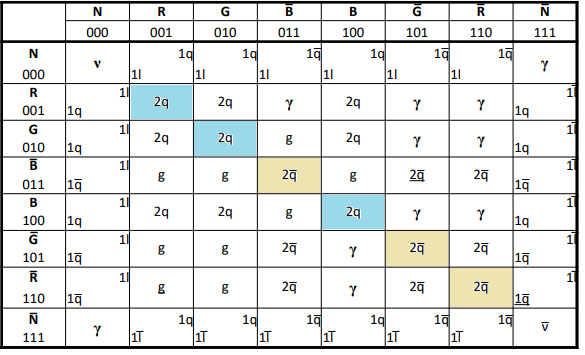
\includegraphics{fig4}
\par\end{centering}
\medskip{}

{\small{}Possible combinations of colored fragments are shown, where (anti)quark fragments are marked $q$ and $\bar{q}$, (anti)neutrinos are $\nu$ and $\bar{\nu}$, gluons are $g$, and photons are $\gamma$. Since half the gluon fragments are right handed, they are shown as photons. The cells marked as blue, if having electric charge $q=+$, may form an }\emph{\small{}up quark}{\small{} fragment in Orbis.}{\small\par}
\end{figure}

%%%%%%%% ENTROPY CONSIDERATIONS %%%%%%%%%%
\section{Entropy Considerations\label{sec:Entropy-considerations}}
At this point, the formal description of the model is considered complete. Let us now examine how the concept of entropy can be used to probe the model for global and local features.

\subsection{Shannon-like entropy}
Shannon entropy provides a measure of the randomness or disorder in a system. For a 3D cellular automaton, it quantifies the uncertainty associated with the system's states. The formula for Shannon entropy, as introduced by Shannon \cite{shannon}, is:

\begin{equation}
H = -\sum p(i) \log_2 p(i),
\label{eq-entropy}
\end{equation}
where \( H \) represents the entropy, \( p(i) \) is the probability of observing a particular state \( i \), and \( \log_2 \) denotes the base-2 logarithm.

\subsection{Defining the state function}
In practice, calculating entropy based on the exact configuration of the entire system is impractical due to the negligible probability of repeated configurations. To address this, we define a \textit{state function} that selects specific properties of interest to represent the state of a cell. These properties include:

\begin{itemize}
    \item \textbf{Spatial Position:} The coordinates \( x, y, z \) of the cell within the lattice.
    \item \textbf{Charge:} A physical property of the cell.
\end{itemize}

These variables are combined into a single numerical value representing the cell's state. Each unique combination of these variables corresponds to a distinct cell state. 

For simplicity, the entropy computation considers only the central cell in each layer (\( W \)) of the 3D lattice. If the cell does not belong to a route, its state defaults to zero.

The total number of possible states is calculated as:
\begin{equation}
N = 64 \times L^3,
\label{eq-nstates}
\end{equation}
where \( L \) represents the lattice size along each dimension.

\subsection{Defining the era}
Entropy is computed over a defined \textit{era}, which represents a segment of the system's evolution. Assume a Poincaré cycle estimated as \( P \) light steps (\( \mathcal{L} \)) is known, and the entropy graph consists of \( WIDTH \) bars. The era is defined as:
\[
\text{era} = \frac{P}{WIDTH}.
\]

\subsection{Calculating entropy}
Entropy is calculated using Equation~(\ref{eq-entropy}) following these steps:

\begin{enumerate}
    \item \textbf{Collect State Occurrences:} Save the state of the central cell in each \( W \)-layer at the end of every light step (\( \mathcal{L} \)).
    \item \textbf{Count State Frequencies:} Record how often each state appears within the lattice over the duration of an era.
    \item \textbf{Determine Probabilities:} Divide the count of each state by the total number of states (\( N \)) to compute its probability \( p(i) \).
    \item \textbf{Compute Entropy:} Apply Shannon's formula (Eqn.~\ref{eq-entropy}) to compute the entropy \( H \).
\end{enumerate}

The resulting entropy values provide insights into the complexity and evolution of the automaton, uncovering patterns and emergent behaviors. Specifically, in the global context, they can help identify the presence of a Poincaré cycle and determine whether information loss prevents the system from returning to its initial state.

%%%%%%%% RESULTS %%%%%%%%%%

\section{Results}\label{sec:Results}

To illustrate the concepts discussed thus far, we have developed a few practical examples.

\subsection{The speed of light and the size of the universe}

We can now state the following constraint on the fundamental quantities:

\[
\frac{X}{\mathcal{L}}=c,
\]
where $c$ is the speed of light and $\mathcal{L}$ is the number of ticks per frame. Estimates for the values of \emph{X} and \emph{L }(truncated to a natural) are taken from Appendix \ref{sec:Calculation-of-X}

\[
X=l_{P}
\]
and

\[
L\approx6.95410\times10^{60}\approx2^{202},
\]
where $l_{P}$ is the Planck length. From this, we calculated the size of the universe as $1.94669\times10^{26}\,m$ (the \emph{Grand Cube} diagonal).

\subsection{A charge conjugation study}

A small program (see Ref. \cite{af_neto}, file \emph{combine.c}) was created to check the combination of charges. A total of $6\times32768=196,608$ fragments, with their charges evenly distributed, were randomly combined in several million attempts and the averages tabulated. It was assumed that only 'hydrogen atoms' are formed.

Since the strong force dominates, a probability value of 0.001 was assigned to the search for up quarks and 0.999 to gluons. These values were calculated based on the smallest possible set of charges. The search was conducted in four stages. First, gluons and up quark fragments were targeted (fragments of electrons were also included, as their existence depends on the number of generated up quarks). Next, photons and neutrinos were sought, followed by fragments of the W and Z bosons, and finally, anti-atoms were examined.

The results can be seen in Table \ref{combina}. The leftover, that is, the bubbles that could not form a pair or a singleton, reveals a highly ionized environment, that will be attenuated by inter-sector
interactions, resulting in an increase in the photon count. These data resemble roughly a few simple 'atoms', while the photon fragments could form a few multiple pair photons. One can then speculate that the unmatched quark fragments could form mesons or virtual quarks or even contribute to dark matter (50\% + 25\%), and that the Umbra contains more antimatter than Orbis. All in all, it makes sense as a toy universe. 

Unfortunately, one key figure for model validation, represented by the proton-electron mass ratio, appears in this simple analysis with a value of just $1187$ for both sectors, rather than the empirical value of $\approx1836$ (CODATA \cite{codata}). 

\begin{table}
\caption{Charge combination}

\medskip{}
\label{combina}
\begin{centering}
{\small{}}%
\begin{tabular}{|l|c|r|r|l|}
\hline 
\textbf{\small{}Fragment} & \textbf{\small{}Type} & \textbf{\small{}Orbis} & \textbf{Umbra} & \textbf{\small{}Obs.}\tabularnewline
\hline 
\hline 
{\small{}Gluon} & {\small{}Pair} & {\small{}3,6760.0} & {\small{}3,6760.0} & \tabularnewline
\hline 
{\small{}Up quark} & {\small{}Pair} & {\small{}42.0} & {\small{}42.0} & \tabularnewline
\hline 
{\small{}Down quark} & {\small{}Single} & {\small{}10.0} & {\small{}10.0} & \tabularnewline
\hline 
{\small{}Electron} & {\small{}Single} & {\small{}31.0} & {\small{}31.0} & \tabularnewline
\hline 
{\small{}Photon} & {\small{}Pair} & {\small{}20.0} & {\small{}20.0} & \tabularnewline
\hline 
{\small{}Graviton} & {\small{}Pair} & {\small{}12.0} & {\small{}12.0} & \tabularnewline
\hline 
{\small{}Z boson} & {\small{}Pair} & {\small{}24,592.0} & {\small{}18,416.0} & \tabularnewline
\hline 
{\small{}W boson} & {\small{}Pair} & {\small{}6,122.0} & {\small{}12,294.0} & \tabularnewline
\hline 
{\small{}Neutrino} & {\small{}Pair} & {\small{}6,082.0} & {\small{}6,082.0} & \tabularnewline
\hline 
{\small{}Antiup} & {\small{}Pair} & {\small{}2.0} & {\small{}2.0} & \tabularnewline
\hline 
{\small{}Antielectron} & {\small{}Single} & {\small{}1.0} & {\small{}0.0} & \tabularnewline
\hline 
{\small{}Antiquark} & {\small{}Single} & {\small{}0.0} & {\small{}0.0} & \tabularnewline
\hline 
{\small{}Leftover} & {\small{}Single} & {\small{}24,624.0} & {\small{}24,620.0} & {\small{}Adds to dark matter}\tabularnewline
\hline 
\textbf{\small{}Total} &  & \multicolumn{2}{r|}{\textbf{\small{}196,602.0 }} & \tabularnewline
\hline 
\end{tabular}{\small\par}
\par\end{centering}
\medskip{}

{\small{}A total of 196,608 bubbles were randomly combined into several million attempts in a small program focused on charges alone (See Sect. \ref{sec:Results} for more details).}{\small\par}
\end{table}


\subsection{Computing the Poincaré cycle}

A highly simplified simulated implementation of the cellular automaton is being developed (see Ref. \cite{af_neto}). Although dimensionally small, it will eventually be fully operational, incorporating all the rules. This model will enable the calculation and visualization of its Poincaré cycle in a straightforward manner.

At first glance, in a closed system like this, entropy is expected to initially increase, followed by a phase of consistent decrease, marking the completion of a full Poincaré cycle. Using the definitions provided in Sect. \ref{sec:Entropy-considerations}, an entropy plot for the model can be generated.

The following section discusses potential challenges and limitations of this approach.

%%%%%%%%%% UNDECIDABILITY %%%%%%%%%%%%%%%%%%%
\section{Undecidability and long-term dynamics}\label{sec-undecidability}

A critical challenge in our model is understanding its long-term dynamics, particularly the determination of a Poincaré cycle. However, the computational complexity underlying its dynamics introduces significant undecidability concerns, especially when scaling the model to larger sizes. Due to its richness, this CA can be computationally equivalent to a Turing machine \cite{wolfram1983}. This equivalence means that certain questions about its evolution, such as predicting whether the system will eventually return to an initial state (a Poincaré cycle) or stabilize, are undecidable \cite{gacs1979}. Specifically, determining if the given initial configuration will lead to periodicity or chaotic evolution cannot be resolved algorithmically. Moreover, increasing the grid size by scaling \( L \) (the linear dimension of the CA grid) exponentially enlarges the configuration space, significantly compounding the complexity of detecting periodic or other predictable behaviors \cite{toffoli1980}.

The \textit{Pigeonhole Principle} guarantees that the system will eventually revisit a previous state, as the number of possible configurations is finite \cite{bernstein2007}. This re-visitation implies that the CA must either stabilize (reach a fixed point) or enter a periodic cycle (a Poincaré cycle). However, the time required to detect periodicity can be exceedingly long, potentially growing exponentially with the grid size \( L \). Although the current scale of the implementation has not yet identified a Poincaré cycle, the undecidability of CA dynamics means that no general method can predict the cycle's length or guarantee that it will be detected \cite{wolfram}.

Constructing a model directly based on these prescriptions may be impractical due to the hierarchical complexity of the problem. If the electromagnetic coupling already imposes a 1/137 factor, the challenges posed by gravitational interactions are even more significant. Therefore, only analytical tools can effectively extract useful insights from the model.

%%%%%%%% PROSPECTS AND CONJECTURES %%%%%%%%%%

\section{Conjectures and prospects\label{sec:Prospects-and-conjectures}}

This work represents the tip of the iceberg. The challenge now is to delve into the many conjectures that emerge from it, prove them, perhaps with minor adjustments.

Just a few examples are considered here.

\subsection{Charge Quantization} \label{subsec:charge-quantization}

A subtle geometric "defect" emerges during the initialization of the CA model (see Section~\ref{initial-state}). When attempting to define the route lines $p$ and twist spirals $\bar{p}$ as isotropically distributed within the lattice's discrete, square-like constraints, unavoidable asymmetries arise. Specifically, the mismatch between the chosen $W$ dimension ($3\cdot L^2$) and the number of isotropic directions ($\pi\cdot L^2$) introduces a structural defect. Rather than being problematic, this defect acts as a useful artifact—enabling the emergence of quantization, in a manner reminiscent of charge quantization in physical systems.

This quantization discretizes the system's possible states, suppressing chaotic evolution and promoting periodic behavior. On smaller grids, it manifests as localized, stable patterns. As the grid scales up, these quantized states remain robust, supporting scalable periodicity and recurring cycles even in larger systems. At this stage, these "islands" of stability become rigidly organized in a highly regular distribution.

A key mathematical foundation for this quantization lies in the concept of the winding number—a topological invariant that counts how many times a vector field wraps around a point or axis. In the CA model, the defect-induced asymmetries naturally associate with a nonzero winding number, effectively enforcing the discreteness of the system’s state space.

To achieve charge quantization—and by extension, the quantization of other fundamental properties—the model requires a mechanism analogous to Dirac's magnetic monopole. In our discrete 3-torus framework, this is realized by ensuring that the property vector $\bar{p}$ exhibits non-trivial winding around at least one of the torus’s non-contractible loops. This behavior mirrors the effect of a magnetic monopole in conventional theories, which enforces the quantization of electric charge \cite{dirac1931}. As a result, the "islands" become even more spatially independent and well-defined.

It is important to note that this quantization is only possible due to the separation between Orbis and Umbra, distinguished by the $w1$ bit (see Section \ref{subsec:all-dirs}). The complementary asymmetries manifest independently within each sector.

Proving this conjecture—and, for instance, calculating the Planck constant from the number of "bubbles" constituting an electron—remains one of the main challenges for future research.

\subsection{Color quantization}
Color quantization is an extension of the electromagnetic case. Hadrons form by the simultaneous action of charge quantization and strong cohesion.

\subsection{Weak quantization}
Due to the relatively rare occurrence of weak interactions, the weak quantization manifests itself at a cosmological scale: the relation between the average distance between galaxies and their bulges is constant. Deriving a cosmological constant $\Lambda$ and the respective metric tensor $g_{\mu\nu}$ from this is an intriguing possibility. 

The large-scale granularity could then also be interpreted as a gravitational quantization.

\subsection{Emergence of gravity}\label{subsec:emergence-of-gravity}

 The smooth spacetime of general relativity is viewed as an effective, coarse-grained approximation of the fundamental discrete structure considered. The model posits that gravity arises as a residual effect of electromagnetic interactions, emerging naturally within the cellular automaton framework through the interplay of photons and gravitons. Acting as super photons, gravitons possess properties that allow them to mediate interactions across the two overlapping sectors of the toy universe, \emph{Orbis} and \emph{Umbra}. While ordinary photons are restricted to sector-specific interactions, gravitons provide a mechanism for fundamental connectivity in a universe otherwise marked by a strong separation between these domains. However, their direct influence on distant masses diminishes due to the cancellation of antagonistic forces (e.g. electric attraction/repulsion) induced by their interactions. What remains is a residual, geometry-driven attractive force \footnote{Recent results confirm that gravity acts attractively on antimatter \cite{anderson2023observation}.} that underpins the emergent gravitational effect, acting locally as described in Section \ref{subsec:special-rel}. Free objects follow emergent timelike geodesics in this scenario. Through this dual-sector capability, gravitons redistribute energy and charge, also contributing to phenomena analogous to dark matter (flat rotation curves of galaxies).

An additional factor in this framework is the gradual energy dissipation observed as photons travel great distances. This \textit{aging} process, intrinsic to the cellular automaton, parallels photon redshift in its effect. As it propagates, an energetic photon undergoes minor interactions with errant singletons and electrons, without collapsing. Over time, this energy dissipation subtly shifts the light spectrum toward the red end.

The idea was first presented by Zwicky in \cite{zwicky1929redshift}, where he was concerned with the blurring of the received images—a phenomenon that does not occur in our model. Could this effect offer an alternative explanation for cosmic redshift, potentially challenging the need for dark energy?

Note that the propeller turns accelerations equivalent, in particular in the case of the proverbial cabin picturing the GR equivalence principle.

\subsection{Stochastic behavior and the uncertainty principle}

The richness of the regular patterns that intersect to determine an interaction, combined with the large number of bubbles that form the particles, results in seemingly random outcomes, despite the deeply deterministic nature of the model. 

This apparent randomness emerges when considering multiple realizations of the same initial conditions, where microscopic variations between individual bubbles lead to a distribution of outcomes. Since both particles and measurement instruments are composed of many bubbles, each measurement effectively samples a single instance from this distribution. Consequently, there will always be a degree of uncertainty in measured values. In quantum mechanics, this uncertainty is fundamental and manifests as the well-known Heisenberg principle \cite{Heisenberg1927}:
\[
\sigma_x \sigma_p \leq \frac{\hbar}{2}.
\]
Here, the standard deviations $\sigma_x$ and $\sigma_p$ represent the spread of position and momentum measurements.

\subsection{Electronic decay}
After the absorption of (part of) a photon, the electron enters an excited state, dynamically stabilizing in a suitable spherical harmonic configuration. When the common components of the photon and electron are re-emitted, the odds of a configuration corresponding to the original photon are less than one. As time passes, after many cohesion interactions, the proper configuration of charges and routes may occur, forming a single photonic blob and allowing the emitted photon to escape the frequent re-emission mechanism, fleeing away from the electron cloud, which eventually settles into its ground state.

\subsection{Black holes}
The quintessential idea of a black hole in this model can be illustrated by two electrons, each with radius $R$, so close to each other $d<2R$ that the quantization is broken and they simply fuse, forming a particle with radius $R'=2^{1/3}R$ with a dominant affinity value. 
\[
a_1 = a_2 = min(A_1,A_2).
\]

A picture of the internals of a black hole can then be readily extrapolated from this simple example: a mixture of bubbles, most lacking quantization while others exhibit it incompletely, in a frenetic and densely packed configuration.

\subsection{The Hofer effect}

A particular challenge is to verify what we call the \emph{Hofer effect,} the expected tendency for all spins of a localized particle to align radially either inward or outward (spin up/down), as predicted in Hofer \cite{hofer}. In that work, there is an explanation of how magnetic effects emerge from symmetry breaking of this spherical pattern, thereby supporting the Stern-Gerlach experiment.

\subsection{Particle zoo panorama}
As mentioned, this is a toy model still under construction, with aspirations to evolve into a full-fledged theory. As is, it serves as a framework to speculate on the composition of known particles in light of the proposed model. In the discussion that follows, the fragments will be characterized by their charge content: \(q, w1, w0, c2, c1, c0\). For example, we designate the fragment \(100000\) as \(-L\) and \(001111\) as \(-\bar{L}\), and so forth.  

\subsubsection{The electron neutrino}
The electron neutrino $\nu_e$ is formed by a single [$+L:-L$] pair and additional propellers. Yet the anti-electron neutrino $\bar{\nu}$ uses the pair [$+\bar{L}:-\bar{L}$].

\subsubsection{The electron}
The electron $e^-$ is formed by a quantized number of $-L$ fragments, a great number of electron neutrinos $\nu_e$ and a variable number of propellers. The positron, or anti-electron, uses $+\bar{L}$ fragments instead. These are for Orbis, in the case of Umbra, all bits are inverted.

\subsubsection{The muon neutrino}
The muon neutrino $\nu_{\mu}$ is formed as $\nu_{\mu}=2\nu_e+\bar{\nu}_e$ plus additional propellers. It is like an electron neutrino, but with a compensated antimatter part.

\subsubsection{The muon}  
The muon $\mu^-$ consists of a quantized number of $-L$ fragments, a large number of muon neutrinos $\nu_{\mu}$, and a variable number of propellers. The classical study conducted by Itô in \cite{ito} suggests that this configuration stabilizes at the second harmonic of the electron's radial vibrational state.

\subsubsection{The tau neutrino}
The tau neutrino $\nu_{\tau}$ is formed as $\nu_{\tau}=3\nu_e+2\bar{\nu}_e$ plus additional propellers. It is also like an electron neutrino, but with a compensated antimatter-enriched part.

\subsubsection{The tau}
The tau $\tau^-$ is formed by a quantized number of $-L$ fragments, a great number of tau neutrinos $\nu_{\mu}$, and a variable number of propellers.

\subsubsection{Leptons decay}
In the Standard Model (SM), the decay products typically include one neutrino or antineutrino. However, in our model, the large number of neutrinos is entangled, sharing a common affinity. When one neutrino interacts via the weak force, all other entangled neutrinos collapse to the same point. This phenomenon gives the appearance of a single, energetic neutrino, as the observable outcome remains indistinguishable, in agreement with the SM predictions.

\subsection{Compound particles half-lives}
Protons, electrons, and electron neutrinos are composed exclusively of bubbles, without their corresponding anti-bubbles. This unique composition is a key factor in their exceptionally long half-lives, potentially making them stable. In contrast, particles containing both bubbles and anti-bubbles are significantly less stable. Their shorter half-lives result from the likelihood of annihilation events between bubbles and anti-bubbles within their structure, leading to their transient nature.

The neutron embeds lots of electron antineutrinos, which bind the negative charge to its inner proton. This explains the decay of the free neutron.
\[
n^0\rightarrow\,p^{+}+e^{-}+\nu_e
\]

\subsection{Heavier quarks}
The framework suggests that the other quarks follow the composition of leptons, with additional neutrinos and antineutrinos, besides a variable number of propellers.

\subsection{Atoms}
Bound states of protons, neutrons, and electrons are naturally expected in this scenario.

\subsection{The abundance of neutrinos}

Despite the relatively small number of neutrinos observed in Table \ref{fig:color-combination}, their large cosmic abundance can be understood in light of their extremely low mass, approximately five million times smaller than the mass of an electron. This characteristic allows neutrinos to exist in enormous quantities across the universe, even if their presence appears limited.

\subsection{Quest for qubits}

An electron may be conceived as a vast number of dynamic microstates, collectively manifesting as a single particle through their underlying affinity. When two electrons share a common affinity, they remain distinguishable only by the constraints of quantization dynamics. Yet, if we momentarily set aside the strict framework of quantization, the pair emerges as a system of qubits, capable of far richer interactions.

The atoms that necessarily host these electrons compartmentalize local space through the SU(3) symmetry induced by the strong charge, further expanding the landscape of possible interactions.

This more fluid perspective suggests that their behavior might resemble an intricate network—or even a swarm—of Turing machines, each representing a potential computational pathway. Such an interpretation could shed new light on the remarkable experimental results emerging from quantum computing, hinting at deeper, perhaps untapped, computational structures within quantum systems.

\section{Cellular automata and quantum formalism} \label{sec:bridge}How can this model be used anyway? At the global level, we have already addressed some of these ideas in Section~\ref{sec:Entropy-considerations}. For local events, our guide to an answer comes from 't Hooft's seminal work about cellular automata as world models \cite{thooft}.

Of course, the ontological states ($\mathcal{OS}$) representing each configuration of the CA cells cannot form superpositions, since ontological states evolve into ontological states. But, an orthonormal set of ontological states can be used as a basis for a Hilbert space, each represented by a unit vector.

Given a subsystem of the universal automaton, the general recipe for analyzing it using operator mechanics is as follows:

\begin{itemize}
    \item Find a permutation operator as a matrix containing a single 1 in any row or column.
    \item Diagonalize it, obtaining the eigenvalues and eigenvector matrices.
    \item Identify a Hamiltonian matrix as the exponent in $\hat{U}=e^{-i\hat{H}T}$.
    \item Use the eigenvalue matrix to bring this Hamiltonian back to the ontological basis.
    \item Form linear combinations of the ontological states $\ket{A}$.
\[
\ket{\psi} = \sum_A \lambda_A \ket{A}, \quad \sum_A |\lambda_A|^2 \equiv 1,
\]
where $\ket{\psi}$ is a quantum state or "template," and $\lambda_A$ is a complex coefficient.
\end{itemize}

Now, we can use the operator mechanics machinery, in particular the Schrödinger equation, to analyze it:

\[
\frac{d}{dt}\ket{\psi} = -i\hat{H}\ket{\psi}.
\]

This is, naturally, a simplified picture. More details can be found in References \cite{thooft,Elze2019,rizzo2020perturbing}.
%%%%%%%% DISCUSSION %%%%%%%%%%

\section{Discussion\label{sec:Discussion}}

\subsection{Novelty of the work}

When compared to previous and ongoing works from Section \ref{sec:related-work}, the novelty of this contribution lies in several key aspects that distinguish it from traditional cellular automata (CA) models and from contemporary computational universe frameworks.

First, the proposed model introduces a non-spatial dimension, $W$, in addition to the conventional three spatial dimensions. This extra dimension is not merely an abstract axis but a dynamic computational layer that enables the convolution of data across different layers (i.e. between particle fragments). While most prior CA models operate solely on spatial configurations and temporal updates, the inclusion of a convolution axis allows for richer interaction dynamics. As a consequence, a superluminal mechanism is naturally required; however, it carries no implications for signaling.

Second, the model incorporates six charge bits from the very beginning, providing a fine-grained internal state space per cell. This stands in contrast with earlier models such as von Neumann’s 29-state automaton or Wolfram’s binary-rule systems, which, despite their expressive power, are often constrained in terms of internal charge representation and conservation. The six-bit encoding allows for nuanced Lie group behaviors reflecting the Noether symmetry–conservation quantity theorem—features emphasized in the works of Margolus and Fredkin but implemented here at a more granular, programmable level.

Third, the unique affinity property groups bubbles into particles, facilitating the aggregation of smaller units into more complex entities. Without it, only a holistic universe would emerge. It is also the substrate for the emergent phenomenon of entanglement and characterizes the track left by the particles in self-interference. There is no similar mechanism in the cited works.

Fourth, the reversibility pursued in the works of Fredkin and Margolus has no place here, because the ontological collapse presented forbids it inside a Poincaré cycle. Actually, reversibility emerges before a collapse happens.

Lastly, while Wolfram’s hypergraph-based model generalizes away from grids, the current work, using a radically different approach, retains a discrete lattice but augments it with multi-layered computational structures, preserving spatial locality while avoiding a highly abstract model. This bridges the gap between a discrete space-time CA model and an emerging theory of quantum and relativistic physics.

These innovations collectively enable new forms of emergent behavior, complexity, and physical interpretation within the CA paradigm, capable of modeling the observed results of experimental physics.

\subsection{Undecidability}
The determination of Poincaré cycles in a finite CA provides valuable insights into the long-term dynamics of toy universe models. However, the undecidability of general CA behavior highlights the limitations of such analyses, particularly when scaling the model to larger sizes. While the periodicity of a smaller system may provide clues about the behavior of a larger system, the introduction of additional degrees of freedom and emergent phenomena makes direct projection challenging.

This interplay between undecidability and scalability reflects the richness and complexity of cellular automata as models for dynamic systems, including hypothetical universes.

\subsection{Observers and spacetime}  

This framework extends Wheeler's "it from bit" concept by providing a mechanism through which information constitutes physical entities, albeit from an omniscient perspective. To address the internal viewpoint, we now define inner observers or simply \textit{observers}. The most accurate description of a system available to such an observer is captured by the epistemic states of Spekkens’ toy theory \cite{Spekkens2007}. Each observer thus operates within an \textit{epistemic horizon}—a fundamental boundary beyond which information is inaccessible. Measurement uncertainty arises naturally from this limited perspective, reflecting the inseparability of subject and object.

As established, the spacetime of this model is inherently flat and regular. However, the spacetime perceived by observers and laboratory instruments appears curved, in accordance with the principles of General Relativity. How can this apparent discrepancy be reconciled?  

The resolution lies in understanding the role of certain dynamic agents, the propellers, which contribute both to motion and to mass-energy content. Their interactions create a framework in which observers, laboratory instruments, and the environment mutually influence one another. This interplay generates effective gravitational potentials, causing clocks to tick slower near concentrations of mass. Such behavior unveils a \textit{timescape} scenario \cite{duley2013timescape}, where the perception of curved spacetime naturally emerges from relational dynamics within an underlying flat background.

Given the mutual dependence of all system components and the absence of free external variables, the model aligns with superdeterministic interpretations of reality, as discussed by Hossenfelder and Palmer \cite{hossenfelder2020rethinking}.

An important philosophical implication then emerges: this model leaves no room for solipsism. The interconnectedness of all components ensures that subjective perspectives are inseparably tied to the system's dynamics, suggesting that relatively independent minds or observers could eventually form naturally anywhere within the system.

\subsection{Falsifiability of the physical model}

A definitive experimental proof that an electron physically traverses two paths in the double-slit experiment would directly contradict the proposed model. Such a finding would demonstrate that self-interference arises not from recorded traces within a structured lattice, but from the electron's simultaneous presence along both paths. Therefore, verifying this dual-path traversal would invalidate the core mechanism of trace-based interference and challenge the assumptions of this discrete lattice model. This testable aspect underscores the model's scientific rigor, providing a clear criterion for falsifiability within the quantum framework.

\subsection{Conclusion}
We are, therefore, facing an ontological,\footnote{Ontology is actually an always receding rule marking the frontier of the unfathomable.} economic framework on a deep subatomic scale. Observable reality is approximate and emergent, possessing continuous spacetime symmetries (Lie, Lorentz, diffeomorphism, CPT, etc.) valid in a wide range. The huge number of bubbles forming the particles --- indeed a mini universe each --- aided by the intrinsic non-locality, gives material support to superposition-like behavior and qubits. These rules can be refined, given sufficient computational power and programming support \footnote{An implementation under development is accessible in Reference  \cite{af_neto}.}, and evaluated if they in fact allow building a predictive, falsifiable, \emph{bona fide,} theory.

Looking ahead, several conjectures were proposed for future research, selected from a wide range of potential ideas.

%%%%%%%% FUNDING %%%%%%%%%%

\section*{Funding and competing interests}
\begin{verbatim}
The author declares that no funds, grants, or other support were received 
during the preparation of this manuscript.

The author has no relevant financial or non-financial interests to disclose.
\end{verbatim}

\printbibliography

%%%% biblio

\newpage{}

%%%%%%%% APPENDIX %%%%%%%%%%

\appendix
\begin{center}
{\LARGE{}Appendix}{\LARGE\par}
\par\end{center}

\section{Calculation of X and L\label{sec:Calculation-of-X}}

Estimates for the value of \emph{X} and the distance between the cells
and \emph{L} (see Sect. \ref{sec:space-and-time}), the granularity
of the grid, will be developed in this appendix.

The diameter of the observable universe \cite{halpbern} is compared
to the diagonal of the lattice.

\begin{equation}
O=8.8\times10^{26}m=\sqrt{3}\,L\cdot X.\label{eq:obs}
\end{equation}
The average photon frequency of CMB \cite{archeops} is

\[
[f]=160\,GHz=160\times10^{6}\,Hz,
\]
which, converted to energy, gives

\[
E=1.060171224\times10^{-25}J.
\]
The proton mass in Joules is

\[
m_{p}=1.503277592969\times10^{17}J,
\]
so, the number of average photons in a proton is

\[
n_{p}=1.4179573\times10^{42}.
\]
The Eddington number gives the number of protons in the universe.

\[
Ed=10^{80}.
\]
Let us calculate the total contribution due to protons in terms of
average photon

\[
n_{pT}=4\,Ed\,n_{p}
\]
or

\[
n_{pT}=5.67183\times10^{122}.
\]
On the other hand, the number of photons in the universe is

\[
n_{\gamma}=4\times10^{84},
\]
which adds almost nothing to the total number due to protons

\[
n_{\gamma T}=n_{\gamma}+n_{pT}=5.67183\times10^{122}.
\]
The wavelength of a single bubble in meters is

\[
\lambda_{0}=L\cdot X
\]
and the frequency of one bubble, in Herz reads

\[
f_{0}=\frac{c}{L\cdot X},
\]
helping to find the number of bubbles in the average photon

\[
n_{b}=\frac{[f]}{f_{0}}=\frac{160\times10^{6}\,L\cdot X}{c}.
\]
So, the amount of bubbles due to all photons is

\[
n_{bT}=n_{b}\,n_{\gamma T}=2\frac{5.67183\times10^{122}\times160\times10^{6}\,L\cdot X}{c}
\]
and

\[
n_{bT}=L^{3}.
\]
We then have

\begin{equation}
\frac{1814.9856\times10^{128}\,X}{c}=L^{2}.\label{eq:number}
\end{equation}
Using Eqn. (\ref{eq:obs}) and Eqn. (\ref{eq:number}), we obtain 

\[
X\approx7.52831\times10^{-24}m
\]
and

\[
L\approx6.74877\times10^{49}.
\]

Assuming that the Planck length is a valid length scale, let us recalculate
$Ed$ for $X=l_{p}$.

\[
Ed=\frac{\sqrt{3}\,c\,O^{2}}{1920\,n_{p}\,l_{p}^{3}}=2.18816\times10^{113}.
\]
Then we finally obtain

\[
X\approx1.616199\times10^{-35}m=l_{p}
\]
and

\[
L\approx6.95410\times10^{60}.
\]

% ALGORITHMS
\newpage{}

\section{Algorithms \label{sec:algorithms}}
Here are grouped the algorithms referenced in the text.

% Algorithm to initialize Euclidean distance

\begin{algorithm}
\caption{Initializing Euclidean distance}
\label{algo:initEuclid}
\begin{algorithmic}[1]
\STATE \textbf{Initialize variables:}
\STATE Set $L$ as the side length of the 3D grid.
\STATE Initialize $count \gets 0$.
\STATE \textbf{Iterate over the grid:}
\FOR{$x = 0$ to $L-1$}
    \FOR{$y = 0$ to $L-1$}
        \FOR{$z = 0$ to $L-1$}
            \STATE \textbf{Calculate offsets:}
            \STATE $dx \gets x - \frac{L}{2}$
            \STATE $dy \gets y - \frac{L}{2}$
            \STATE $dz \gets z - \frac{L}{2}$
            \STATE \textbf{Compute Euclidean distance:}
            \STATE $d \gets \sqrt{dx^2 + dy^2 + dz^2}$
            \IF{$L/2 \leq d < L/2 + 1$}
                \STATE Increment $count$ by 1
            \ENDIF
        \ENDFOR
    \ENDFOR
\ENDFOR
\STATE \textbf{Additional iteration until `count` reaches threshold:}
\FOR{$x = L-1$ \textbf{down to} $0$}
    \IF{$count < 3 \cdot L^2$}
        \FOR{$y = 0$ to $L-1$}
            \FOR{$z = 0$ to $L-1$}
                \STATE \textbf{Calculate offsets:}
                \STATE $dx \gets x - \frac{L}{2}$
                \STATE $dy \gets y - \frac{L}{2}$
                \STATE $dz \gets z - \frac{L}{2}$
                \STATE \textbf{Compute Euclidean distance:}
                \STATE $d \gets \sqrt{dx^2 + dy^2 + dz^2}$
                \IF{$L/2 \leq d < L/2 + 1$}
                    \STATE Increment $count$ by 1
                \ENDIF
            \ENDFOR
        \ENDFOR
    \ENDIF
\ENDFOR
\end{algorithmic}
\end{algorithm}

% Algorithm to initialize points on a sphere
\begin{algorithm}
\caption{Generate uniform points on the sphere surface with constraint}
\label{alg:generateSpherePoints}
\begin{algorithmic}[1]
\STATE \textbf{Input:} Radius $R$, Number of points $u$, Selection parameter $L$
\STATE \textbf{Output:} List of selected points on the sphere surface
\STATE Initialize an empty list \texttt{points}
\FOR{$i = 0$ to $u-1$}
    \STATE Compute $\phi \gets \arccos(1 - 2 \cdot \frac{i + 0.5}{u})$
    \STATE Compute $\theta \gets \pi \cdot (1 + \sqrt{5}) \cdot i$
    \STATE Compute Cartesian coordinates:
    \STATE \hspace{1em} $x \gets R \cdot \sin(\phi) \cdot \cos(\theta)$
    \STATE \hspace{1em} $y \gets R \cdot \sin(\phi) \cdot \sin(\theta)$
    \STATE \hspace{1em} $z \gets R \cdot \cos(\phi)$
    \STATE Compute weight $w \gets \sin^3(\theta)$
    \STATE Add point $(x, y, z, w)$ to the list \texttt{points}
\ENDFOR
\STATE Sort \texttt{points} by $w$ in descending order
\STATE Select the first $N = 3L^2$ points
\STATE Round the selected points
\STATE Remove duplicates
\RETURN \texttt{points}
\end{algorithmic}
\end{algorithm}


% Algorithm to initialize momentum

\begin{algorithm}
\caption{Initialize route vectors}
\label{algo:initPoleVectors}
\begin{algorithmic}[1]
\STATE // C is the center of the lattice; d2 is the distance squared 
\STATE $r_{\text{max}} \gets \text{C}$
\STATE $n_{\text{steps}} \gets \text{C}$
\STATE $\text{step\_size} \gets 1.0 / n_{\text{steps}}$
\STATE $\text{center\_cell} \gets \text{lattice}[\text{C}][\text{C}][\text{C}][0]$
\STATE $w \gets 0$ // Counter for initialized vectors
\FOR{$x \gets 0$ to $\text{SIDE} - 1$}
    \FOR{$y \gets 0$ to $\text{SIDE} - 1$}
        \FOR{$z \gets 0$ to $\text{SIDE} - 1$}
            \STATE $dx \gets x - \text{C}$, $dy \gets y - \text{C}$, $dz \gets z - \text{C}$
            \STATE $\text{d2} \gets dx^2 + dy^2 + dz^2$
            \FOR{$i \gets 0$ to $n_{\text{steps}} - 1$}
                \STATE $\text{lower} \gets r_{\text{max}} - 1 + i \cdot \text{step\_size}$
                \STATE $\text{upper} \gets r_{\text{max}} - 1 + (i + 1) \cdot \text{step\_size}$
                \STATE $\text{lower\_sq} \gets \text{lower}^2$
                \STATE $\text{upper\_sq} \gets \text{upper}^2$
                \IF{$\text{d2} \geq \text{lower\_sq}$ \textbf{and} $\text{d2} < \text{upper\_sq}$}
                    \STATE $p \gets [x, y, z]$
                    \STATE $\text{momenta}[w] \gets p$
                    \STATE $w \gets w + 1$
                    \IF{$w = W_{\text{DIM}}$}
                        \RETURN
                    \ENDIF
                \ENDIF
            \ENDFOR
        \ENDFOR
    \ENDFOR
\ENDFOR
\end{algorithmic}
\end{algorithm}

\begin{algorithm}
    \caption{Convolution algorithm - Part 1}
    \label{algo:convolution1}
    \begin{algorithmic}[1]
        \IF{$T1=D1$ \textbf{and} $T2=D2$}
            \STATE Wavefronts active 
            \IF{$X1 = X2$}
                \STATE Superposition
                \IF{$CH1 = \overline{CH2}$}
                    \STATE Segregation
                    \STATE \textbf{Relocate()}
                \ELSIF{$F1 = 1$ \textbf{and} $F2 = 1$}
                    \IF{Pair is legal}
                        \IF{Gluon pair}
                            \STATE $A1 = A2 = \max(A1, A2)$
                            \STATE $F1 = F2 = 2$
                            \STATE \textbf{Relocate()}
                        \ELSE
                            \STATE $A1 = A2 = \max(A1, A2)$
                            \STATE $F1 = F2 = 2$
                            \STATE \textbf{Relocate()}
                        \ENDIF                            
                    \ENDIF   
                \ELSIF{$F1 > 1$ \textbf{and} $F2 > 1$}
                    \IF{Multi-pair legal}
                        \STATE $A1 = A2 = \max(A1, A2)$
                        \STATE $F1 = F2 = F1 + F2$
                        \STATE \textbf{Relocate()}
                    \ENDIF   
                \ENDIF   
            \ELSE
                \STATE See Algorithm \ref{algo:convolution2} for distinct case
            \ENDIF   
        \ENDIF   
        \STATE  % Creates an empty line
        \STATE \textbf{Legend:}
        \STATE Bubble $1$ is in the current lattice.
        \STATE Bubble $2$ is in the mirror lattice.

    \end{algorithmic}
\end{algorithm}

\begin{algorithm}
    \caption{Convolution algorithm - Part 2}
    \label{algo:convolution2}
    \small
    \begin{algorithmic}[1]
        \IF{$CH1=\sim CH2$}
            \STATE Singularization
            \STATE $F1=F2=1$; $A1=W1;\,A2=W2$
            \STATE \textbf{Relocate()}
        \ELSIF{$F1=1$ \textbf{and} $F2=1$}
            \IF{$COLOR1=COLOR2$}
                \STATE Quark cohesion
                \STATE $A1=A2=\max(A1, A2)$
                \STATE \textbf{Relocate()}
            \ELSIF{$pole1$ \textbf{and} $route2$ \textbf{and} $W1=W2$  \textbf{and}  $CH1=\sim CH2$}
                \STATE Annihilation
                \STATE $F1=F2=1$; $A1=W1;\,A2=W2$
                \STATE Collapse
                \STATE \textbf{Relocate()}
            \ELSIF{($route1$ \textbf{or} $twist1$) \textbf{and} ($route2$ \textbf{or} $twist2$)}
                \IF{electron x electron}
                    \STATE Electron Cohesion
                    \STATE $A1=A2=\max(A1, A2)$
                    \STATE \textbf{Relocate()}
                \ELSIF{electron x electron track}    
                    \STATE Electron self-interference
                    \STATE \textbf{Relocate() just the electron}
                \ENDIF    
            \ENDIF   
        \ELSIF{$F1=1$ \textbf{and} $F2>1$}
            \IF{opposite collors}
                \STATE Quark x gluon
                \STATE \textbf{Relocate()}
            \ELSIF{$sine1$ \textbf{and} $sine2$ \textbf{and} $A1\neq W$}
                \IF{E.M. interaction \textbf{and} $A1\neq A2$}
                    \STATE Light-matter interaction
                    \STATE Collapse
                    \STATE \textbf{Relocate()}
                \ELSIF{Weak interaction \textbf{and} $A1\neq A2$}
                    \STATE Fermion x weak boson OR fermion x neutrino
                    \STATE \textbf{Relocate()}
                \ENDIF        
            \ELSIF{$route1$ \textbf{and} $route2$}
                \STATE Coulomb force
                \STATE \textbf{Relocate()}
            \ELSIF{$twist1$ \textbf{and} $twist2$}
                \STATE Magnetism
                \STATE \textbf{Relocate()}
            \ENDIF   
        \ELSIF{$F1>1$ \textbf{and} $F2>1$}
            \IF{Strong interaction}
                \STATE Gluon x gluon
                \STATE \textbf{Relocate()}
            \ELSIF{Weak}
                \STATE Weak boson cohesion
                \STATE \textbf{Relocate()}
            \ENDIF   
        \ENDIF   
    \end{algorithmic}
\end{algorithm}

\end{document}
